\documentclass[12pt, oneside, a4paper]{book}

% UTF-8 kódovanie pre vstup
\usepackage[utf8]{inputenc}

% slovenčina
\usepackage[slovak]{babel}

% riadkovanie 1,5
\usepackage[onehalfspacing]{setspace}

% referencie
\usepackage[
  backend=biber,
  hyperref=true,
  url=true,
  maxcitenames=2,
  citestyle=authortitle,
  bibstyle=authortitle,
  autocite=footnote,
  language=english % toto mi dá poslovenčený názov (nechápem, ale funguje)
]{biblatex}

% generované Mendeleyom
\addbibresource{library.bib}

% aby fungovali podjebníky v linkoch
\DeclareSourcemap{
 \maps[datatype=bibtex]{
   \map{
     \step[fieldsource=url,
       match=\regexp{\\_},
       replace=\regexp{_}]
   }
 }
}

% okraje
\usepackage[
  top=2.5cm,
  bottom=2.5cm,
  left=3.5cm,
  right=2.0cm
]{geometry}

% obrázky
\usepackage{graphicx}
\graphicspath{{obrazky/}}

% fonty
\usepackage[T1]{fontenc}
\usepackage{lmodern}
%\usepackage[light,math]{iwona}
%\usepackage{inconsolata}
%\usepackage{charter}
%\usepackage[bitstream-charter]{mathdesign}
\usepackage{gensymb} % na \degree
 
% klikateľné referencie a linky
\usepackage[
  unicode=true,
  breaklinks=true
]{hyperref}
\hypersetup{colorlinks=false}

% 
\usepackage{tocbibind}

% matika
\usepackage{amsmath}
\usepackage{amssymb}

% zdrojáky
\usepackage{listings}
\lstset{
  basicstyle=\footnotesize\linespread{0.94}\ttfamily,
  numbers=left,
  xleftmargin=2\parindent
}
\usepackage{multicol}
\usepackage{totpages}

% lepšie odkazy
%\usepackage{url}

\usepackage{float}
\usepackage[bottom]{footmisc}
\usepackage{wrapfig}
\usepackage{lscape}
\usepackage{rotating}
\usepackage{epstopdf}

% nejaké definície pre obal, titulný list, atď.
\def\university{Univerzita Komenského v Bratislave}
\def\universityShort{UK}
\def\faculty{Fakulta matematiky, fyziky a informatiky}
\def\facultyShort{FMFI}
\def\studyProgramme{Kognitívna veda}
\def\branchOfStudy{9.2.11 Kognitívna veda}
\def\educationalDepartment{Centrum pre kognitívnu vedu}
\def\thesisTitle{Nástroj na interaktívne experimentovanie\\s umelými neurónovými sieťami}
\def\thesisSubtitle{Podtitul práce}
\def\thesisType{Diplomová práca}
\def\author{Bc.~Milan Lajtoš}
\def\authorAbstract{LAJTOŠ, Milan}
\def\advisor{RNDr.~Kristína Rebrová~PhD.}
\def\place{Bratislava}
\def\date{2014}

\begin{document}
 
% žiadna hlavička stránky
\pagestyle{plain}
 
% úvodná časť
\frontmatter

% obal
\thispagestyle{empty}

\begin{center}
\Large \textsc{\university\\\faculty}
\end{center}

\vfill

\begin{center}
\Large \textsc{\thesisTitle}\\
\bigskip
\bigskip
\large \textsc{\thesisType}
\end{center}

\vfill

\begin{center}
\large
\textsc{\date}
\hfill
\textsc{\author}
\end{center}

% obal nepočítame do strán
\setcounter{page}{0}

% titulny list
% názov vysokej školy, 
% názov fakulty, 
% názov a podnázov (ak sa podnázov použil), 
% označenie školského diela (diplomová práca)
% meno, priezvisko a tituly autora, 
% názov študijného programu
% číslo študijného odboru vo forme prvého štvorčíslia kódu podľa osobitného predpisu a názov študijného odboru,
% meno, priezvisko a tituly vedúceho práce, resp. školiteľa
% meno, priezvisko a tituly konzultanta, ak bol určený
% školiace pracovisko (ak bolo určené), 
% miesto a rok predloženia. 

\newpage
\thispagestyle{empty}

\begin{center}
\Large \textsc{\university}\\
\Large \textsc{\faculty}
\end{center}

\vfill

\begin{center}
\Large \textsc{\thesisTitle}\\
\bigskip
\bigskip
\large \thesisType
\end{center}

\vfill

\begin{tabbing}
Študijný program: \quad \quad \= \studyProgramme\\
Študijný odbor: \> \branchOfStudy\\
Školiace pracovisko: \> \educationalDepartment\\
Školiteľ: \> \advisor
\end{tabbing}

\bigskip
\bigskip
\bigskip

\begin{center}
\large
\place\ \date
\hfill
\author
\end{center}

% zadanie
\chapter{Zadanie}

\section*{Anotácia}
Umelé neurónové siete sú jedným z najčastejšie používaným modelovacím nástrojom v kognitívnej vede. Patria medzi povinnú literatúru aj v doméne umelej inteligencie. Často ich však ľudia považujú za niečo príliš zložité až mysteriózne, pretože pre ich kompletné porozumenie je potrebné ovládať zložitú matematiku a pre ich implementáciu zas programovanie na určitej úrovni.

Napriek tomu, že v modernej kognitívnej vede dominuje prístup spoznávania pomocou skúsenosti, paleta grafických demonštračných nástrojov na výuku neurónových sietí je stále pomerne chudobná. Ideálnym médiom pre vytvorenie platformy pre demonštráciu neurónových sietí je teraz už všade dostupný web. S pokrokom webových technológií a programovacích jazykov prichádza aj dobrá možnosť pre vznik výučbového prostredia pre online vytváranie a trénovanie neurónových sietí.

\section*{Cieľ}
V teoretickej časti práce, študent priblíži model umelého neurónu a typy umelých neurónových sietí, v ktorých sa takýto neurón používa. V súlade s nadobudnutými poznatkami z kognitívnej psychológie, študent navrhne softvérové prostredie, v ktorom možno interaktívne experimentovať s takýmito sieťami. Následne v praktickej časti práce, študent naimplementuje navrhnutý softvérový nástroj schopný demonštrácie rôznych typov sietí na vybranom probléme.

\section*{Literatúra}

\begin{enumerate}
  \item \cite{Rojas96}
  \item \cite{Johnson2010}
  \item \cite{Victor2013}
\end{enumerate}

% abstrakt v slovencine a anglictine
\chapter{Abstrakt}

\authorAbstract: Nástroj na interaktívne experimentovanie s umelými neurónovými sieťami\ [Diplomová práca]. \university. \faculty; \educationalDepartment. Vedúci diplomovej práce: \advisor, \place: \facultyShort\ \universityShort, \date. \ref{TotPages}~s.

\bigskip

Táto práca sa zaoberá biologicky-inšpirovaným výpočtovým modelom -- umelými neurónovými sieťami. Argumentujeme, že hlboké neurónové siete sú perspektívny výpočtový model a poukazujeme na fakt, že jeho využitie je silne obmedzené nástrojmi, ktoré poskytujú túto funkcionalitu. Tvrdíme, že treba nové nástroje, ktoré nám pomôžu vytvárať a porozumieť systémom, ktoré sú založené na umelých neurónových sieťach. Popisujeme tri princípy, ktoré by mali byť dodržané pri vytváraní takéhoto prostredia a predstavujeme prototyp, v ktorom sú tieto princípy implementované.

\bigskip

\noindent Kľúčové slová: strojové učenie, hlboké neurónové siete, vizuálne programovanie

\chapter*{Abstract}

\authorAbstract: Interactive Experimentation Tool for Artificial Neural Networks [Master Thesis]. Comenius University in Bratislava. Faculty of Mathematics, Physics and Informatics; Centre for Cognitive Science. Master Thesis Supervisor: \advisor, \place: \facultyShort\ \universityShort, \date. \ref{TotPages}~p.

\bigskip

This thesis deals with biologically-inspired computational model -- artificial neural networks. We argue that deep neural networks are a prospective computational model, and we point out that its application is heavily limited due to tools, which provide this functionality. We claim there is a need for new tools which can help us create and understand systems based on the neural networks. We define three principles, which should be adhered to when conceiving such environment, and we present a prototype which implements these principles.

\bigskip

\noindent Keywords: Machine Learning, Deep Neural Networks, Visual Programming

% predhovor
\chapter{Predhovor}

Príchod strojovej inteligencie je len otázkou času. Aby sme tento čas skrátili, potrebujeme nástroje, ktoré nám umožnia \emph{vytvárať a porozumieť systémom}, ktoré sú medzistupňom k skutočnej strojovej mysli.

Táto záverečná práca pojednáva o takomto nástroji a princípoch, ktoré by mal spĺňať. Tiež predstavuje prototyp, ktorý vznikol aplikáciou spomínaných princípov na oblasť umelých neurónových sietí, ktoré sú v oblasti strojového učenia najperspektívnejší model ľudskej kognície.

\bigskip

Toto dielo by nevzniklo bez podpory, ktorej sa mi za uplynulý čas dostalo. Chcel by som sa poďakovať RNDr.~Kristíne Rebrovej~PhD. za ničím neobmedzený priestor pri tvorbe tejto práce. Rovnako by som sa chcel poďakovať aj Slnku môjho života, ktoré mi rozjasňuje každý jeden deň a aj každú jednu noc, a teda mi nedá spávať. Avšak najväčšia vďaka patrí mojej rodine, bez ktorej by nič z tohto nebolo možné a ani nutné.

\vfill

\begin{quote}
\Large
What I cannot create, I do not understand.\\
\mbox{}~\hfill \large Richard Feynman
\end{quote}


\vfill

% obsah
\tableofcontents

% zoznam ilustracii
\listoffigures

% hlavná textová časť
\mainmatter{}

% hlavný obsah práce

% ÚVOD

\chapter*{Úvod}
\addcontentsline{toc}{chapter}{Úvod}

Cieľom výskumu v oblasti umelej inteligencie, je vytvoriť umelú myseľ. Táto myseľ sa musí správať ako dokonalá čierna skrinka -- žiadne nastaviteľné parametre, žiadne ladenie a žiadne vnútorné zásahy. Skutočne samostatný \emph{mysliaci stroj}. Samozrejme, toto potrvá ešte nejaký čas\dots Medzitým potrebujeme nástroje, ktoré nám umožnia vytvárať a porozumieť systémom, ktoré sa stanú predchodcami k skutočnej strojovej mysli.

Nástroje, ktoré nám umožňujú vytvárať systémy imitujúce inteligentné správanie, si zvyčajne vyžadujú akademické znalosti na hranici ľudského poznania. Tieto vedomosti sú častokrát nedostupné alebo zabalené vo forme, ktorá nie je prístupná väčšine ľudí. Ak chceme výskum v oblasti umelej inteligencie urýchliť, potrebujeme nástroje, ktoré umožňujú experimentovanie s takýmito systémami len s minimálnymi znalosťami.

Oblasť hlbokých neurónových sietí je sľubná cesta, ktorá poskytuje mimoriadne výsledky na mnohých úlohách strojového učenia ako napr. rozpoznávanie vizuálnych vnemov, rozpoznávanie reči, predikcia molekulárnej aktivity a ďalších. Avšak na použitie tohto výpočtového modelu sú potrebné matematické znalosti a schopnosť programovať.

Tieto prekážky sa dajú obísť, keď budeme používať nástroj, ktorý nám umožní vytvárať a porozumieť neurónovým sieťam prirodzenejším spôsobom ako symbolickými reprezentáciami, ktoré používa matematika a programovanie. Tento nástroj musí klásť dôraz na všetky tri stupne mentálnych reprezentácií -- na enaktívne, ikonické a symbolické. Teda musí poskytovať rozhranie pre akcie, obrazy a symboly.

Vizuálne programovanie umožňuje používateľom vytvárať programy grafickou manipuláciou prvkov, namiesto písania zdrojového kódu programu. Takéto prostredie je založené na myšlienke \uv{krabíc a šípok}, kde krabice predstavujú entity a šípky vzťahy medzi nimi. Paradigma vizuálneho programovania je častokrát používaná na návrh komplexných systémov a teda je vhodnou voľbou na vytváranie neurónových sietí.

Vizuálne programovanie trpí rovnakým problémom ako písanie zdrojového kódu -- človek iba slepo narába so symbolmi. Vizuálne programovanie neprináša žiadnu pridanú hodnotu oproti tradičnému programovaniu. Tento problém môže byť odstránený zobrazením dát, ktoré prúdia cez sieť. Rozdiel v týchto dvoch prístupoch je porovnateľný s rozdielom medzi MRI a fMRI zobrazovacími technikami. Porozumenie architektúre nie je dostatočné na vysvetlenie dejov, odohrávajúcich sa v tomto dynamickom systéme.

\subsubsection{Členenie práce}

Táto práca je delená na 3 kapitoly. V prvej kapitole popisujem historické snaženie o vytvorenie umelej mysle. V druhej kapitole sa nachádzajú teoretické základy ohľadom konekcionistického modelovania kognitívnych procesov. V tretej kapitole predstavené prostredie na vytváranie neurónových sietí a aj popisané možné pokračovanie týchto myšlienok.

%   MODEL MYSLE

\chapter{Model mysle}

\section{Výpočet}

Historicky najhlbší vhľad do podstaty myslenia nám ponúkol v 17. storočí René Descartes. Tvrdil, že myšlienky sú len \emph{symbolické reprezentácie} analogické k matematickým reprezentáciám, t.j. mentálne reprezentácie a objekty, ktoré reprezentujú môžu byť oddelené. V tomto rámci uvažovania myslenie nie je nič iné ako manipulácia symbolických reprezentácií -- \emph{výpočet}. \autocite[str. 31]{Petru2007}

Thomas Hobbes, Descartov súčasník, tiež došiel k záveru, že myslenie má matematickú podstatu. Opísal ju nasledovne:
\begin{quote}\uv{Ak niekto myslí, nerobí nič iné ako že si predstavuje celkový súčet sčítaním častí alebo zbytok odčítaním jedného súčtu od iného.}\autocite[kap. 5, O rozumu a věde]{Hobbes2009} \end{quote}

Ak sa tejto definície pridržíme, otázka \emph{umelej mysle}, resp. stroja vykonávajúceho myslenie, príde sama od seba.

\section{Mysliace stroje}

Idea, že myslenie sa dá redukovať na sériu výpočtov, je z rôznych pohľadov veľmi zaujímavá. Ak predpokladáme jej pravdivosť, tak by bolo možné zostrojiť mechanizmus, ktorý by takýto výpočet vykonával -- \emph{mysliaci stroj}.

Využitie takéhoto stroja je pomerne neobmedzené, pretože môže vykonávať akúkoľvek \emph{myšlienkovú} činnosť, ktorú zvládne človek. Prvá možnosť ako by sa takýto stroj dal využiť je, že by mohol myslieť za nás. Oslobodil by nás tak od námahy, ktorú musíme denne podstupovať.

Na druhej strane, vo svetle Descartovho výroku \emph{\uv{Myslím teda som}}, naberá predstava stroja, ktorý myslí za nás, zvláštny rozmer. Ak by sme už nemuseli myslieť, prestali by sme existovať? Tento názor nás paradoxne núti zamyslieť sa a \emph{byť} ešte viac.

Najvhodnejším spôsobom ako sa pozerať na mysliace stroje je považovať ich za predĺženie ľudskej mysle. Podobne ako nám rôzne nástroje umožňujú znásobiť vrodené schopnosti, tak nám umelá myseľ môže otvoriť dvere, o ktorých sme ani nevedeli, že existujú\dots

\section{Počítacie stroje}

\subsection[História]{História počítacích strojov}

História počítacích strojov obsahuje množstvo osobností a ich objavy, ktoré posunuli poznanie podstaty výpočtu veľkými skokmi dopredu.

\subsubsection{Počítacie hodiny}

Úplne prvý počítací stroj zostrojil Wilhelm Schickard v roku 1623. Schickardov stroj používal ozubené kolieska pôvodne určené pre hodiny, preto sa jeho vynález niekedy označuje ako \uv{počítacie hodiny}. Aj napriek faktu, že tento stroj vedel iba sčítavať a odčítavať čísla, našiel si praktické využitie -- Johanes Kepler ho použil pri svojich astronomických výpočtoch.

Schickard prišiel s myšlienkou počítacieho stroja ako prvý, avšak ako to už býva zvykom, byť prvý častokrát nestačí. Tam kde všetko začalo, aj všetko skončilo.

\subsubsection{Pascalina}

Nezávisle od Schickarda, Blaise Pascal v roku 1642 zhotovil počítací stroj nazvaný Pascalina. Rovnako ako jeho predchodca, tento stroj vedel iba sčítavať a odčítavať. Pascal však urobil jeden zásadný krok, ktorý ho odlíšil od Schickarda.

Pascalov dizajn počítacieho stroja bol natoľko bezchybný, že sa rozhodol rozšíriť svoj vynález medzi ľudí, čo malo rôzne následky. Spoľahlivosť Pascaliny ohromila úradníkov až do takej miery, že sa začali obávať o stratu svojho zamestnania.

Pascal mal viac šťastia ako Schickard, jeho dielo inšpirovalo ďalšie generácie, ktoré myšlienku počítacieho stroja posunuli vpred.

\subsubsection{Leibnizov projekt}

Ďalším krok v histórii počítacích strojov učinil Wilhelm Gottfried von Leibniz v roku 1694. Leibniz zdokonalil Pascalov dizajn a vytvoril počítací stroj, ktorý navyše vedel násobiť a aj deliť.

Leibniz mal však rozpracovaný väčší plán, ktorý mal priniesť skutočný mysliaci stroj, nie iba pomôcku na počítanie. Aj napriek tomu že neuspel, zanechal svojím pokračovateľom základy, ktoré sa stali kľúčové pri plnení jeho sna.

\subsubsection{Analytický stroj}

Pokračovateľom Leibnizovej myšlienky bol Charles Babbage, ktorý zostrojil Diferenčný stroj. Ten umožňoval počítať s polynomiálnymi funkciami, čo mnohonásobne zvyšovalo použitie stroja v rôznych oblastiach matematiky.

Babbage cítil obmedzenia svojho vynálezu, no vytrval a v roku 1837 opísal stroj, ktorý by umožňoval vypočítať čokoľvek -- Analytický stroj. Myšlienka tohto stroja predstihla možnosti svojej doby a kvôli technickým problémom Babbage svoju prácu nikdy nedokončil.

\subsubsection{Elektronická kalkulačka}

Predchádzajúce stroje uskutočňovali výpočet čisto mechanicky -- otáčali ozubenými kolesami. George Stibitz toto zmenil, keď v roku 1937 dokončil prvý číslicový počítací stroj, ktorý používal elektromagnetické spínače. Vďaka elektronickým súčiastkam bol Stibitzov stroj podstatne rýchlejší ako dovtedajšie pokusy o počítacie stroje.

\subsubsection{Turingov stroj}

V roku 1937 bol predstavený ďalší počítací stroj, ktorý však nemal fyzickú formu. Tento teoretický stroj vymyslel Alan Turing, ktorý priamo nadviazal na Babbageov Analytický stroj.

Hlavnou charakteristikou Turingovho stroja je zapisovateľná \emph{páska}, \emph{hlava}, ktorá sa pohybuje po páske a \emph{strojová tabuľka} s pravidlami. Činnosť Turingovho stroja sa dá popísať nasledovne:
\begin{enumerate}
  \item stav stroja a hodnota z aktuálneho políčka pásky udávajú vstupnú konfiguráciu
  \item strojová tabuľka obsahuje mapovanie zo vstupnej konfigurácie na výstupnú konfiguráciu
  \item výstupná konfigurácia udáva novú hodnotu zapísanú na pásku, posun pásky v istom smere a zmenu stavu
\end{enumerate}

Na prvý pohľad sa zdá, že tento stroj je príliš jednoduchý na to, aby mohol vykonávať akúkoľvek zmysluplnú činnosť, nie to ešte myslieť. Avšak Turing dokázal, že jeho stroj je schopný akéhokoľvek výpočtu.\autocite{Turing1936}

Turing navyše ukázal, že je možné zostrojiť stroj s takou tabuľkou, ktorý dokáže simulovať všetky iné stroje. Tento \emph{univerzálny Turingov stroj}, prečíta z pásky strojovú tabuľku iného stroja a vykoná operácie presne tak ako by ich vykonal popísaný stroj.

Turing svojím objavom otvoril Pandorinu skrinku. Na uskutočnenie umelej mysle už nebolo potrebné konštruovať zložité mechanizmy, stačilo by nájsť tú \emph{správnu} strojovú tabuľku.

\subsubsection{ENIAC a pokračovatelia}

Prvý čisto elektrický počítací stroj, ktorý bol schopný vykonať akúkoľvek vypočítateľnú funkciu, bol ENIAC v roku 1946.\footnote{Babbageov Analytický stroj by bol prvým mechanickým. Prvý elektro-mechanický postavil Konrad Zuse už v roku 1941.} Od tohto momentu sa výpočtový svet zmenil už iba málo.

Poslednú veľkú zmenu do počítacích strojov priniesol EDVAC, na ktorého vývoji sa podieľal aj John Von Neumann. Narozdiel od ENIAC-u používal dvojkovú sústavu namiesto desiatkovej. EDVAC priniesol aj zmenu v nastavovaní strojovej tabuľky. Kým ENIAC musel byť programovaný použitím prepínačov a spojovacích káblov, EDVAC mal strojovú tabuľku uloženú v pamäti, teda podobne ako univerzálny Turingov stroj. Architektúra zavedená Von Neumannom je používaná dodnes.

\subsubsection{Súčasnosť}

Za posledných sedem desaťročí sa udialo vo výpočtovom svete mnoho objavov, ktoré posúvajú hranice stále ďalej. Ako tvrdí Moorov zákon, exponenciálny rast výpočtovej sily stále pokračuje a nezdá sa, že by sa v tomto ohľade malo niečo zmeniť. Výpočtové stroje budú rýchlejšie, menšie, úspornejšie a lacnejšie. Dôsledkom tohto trendu bude vytvorenie paralelne distribuovaného systému vytvoreného z jednoduchých výpočtových jednotiek, ktoré sú extrémne efektívne.

Počítacie stroje majú za sebou dlhú históriu počas ktorých prešli podstatnými zmenami, avšak v ich najhlbšej podstate stále ostávajú rovnocenné univerzálnemu Turingovmu stroju. A to sa týka nielen výpočtovej sily, ale aj problémov s nastavovaním ich strojovej tabuľky\dots

\subsection{Programovanie}

Počítací stroj, resp. počítač, ktorý dokáže vykonať akúkoľvek vypočítateľnú funkciu, je v mnohých smeroch výhrou. Avšak kde sa jeden problém vyrieši, tam vznikne ďalší, doplnkový. Tento problém sa týka nastavenia strojovej tabuľky výpočtového stroja, teda \emph{problém programovania} počítača.

Návod ako vypočítať nejakú funkciu -- algoritmus, musí vložiť do stroja človek -- programátor. Táto úloha si vyžaduje programátorov vhľad do riešeného problému, ale aj schopnosť previesť riešenie do formy zrozumiteľnej pre počítač. Na obe tieto činnosti musí človek vynaložiť námahu, ktorej nás mali počítače zbaviť.

\subsubsection{Spôsob programovania}

Prvé  počítače boli programované na tej najnižšej možnej úrovni. Na zmenu ich činnosti boli používané \emph{prepínače} a \emph{spojovacie káble}. Nastavenie počítača a vyriešenie problému boli dve odlišné veci. Programátor napísal program na papier, ktorý bol predaný operátorom počítača a tí nastavili počítač do želaného stavu.

Príchodom \emph{uloženého programu} sa programovanie podstatne zjednodušilo. Úloha programátora a operátora počítača sa zlúčila, čím došlo k užšiemu prepojeniu medzi programátorom a programovaným. Programátor zapísal sled inštrukcií na úložné médium a počítač ich po prečítaní vykonal. Takýto program musel byť napísaný v strojovom kóde počítača, teda programátor si musel prispôsobiť myslenie strojovým reprezentáciám.

Veľkú zmenu priniesol špeciálny program, ktorý vedel vytvárať iné programy -- \emph{kompilátor}. Kompilátor, resp. prekladač, dokáže preložiť program z formy zrozumiteľnej človeku do strojového kódu. Program mohol nadobúdať rôznu podobu, ktorá však musela dodržiavať pravidlá, ktoré diktoval \emph{programovací jazyk}. Programátor už nie je nútený prispôsobiť sa stroju a môže sa vyjadrovať spôsobom, ktorý je bližší ľudskému mysleniu.

Ako poznáme množstvo vzorov myslenia, tak existujú aj rôzne štýly programovania. Napríklad, dlho sa verilo, že rozmýšľame v logických krokoch, preto vznikli programovacie jazyky, ktoré využívali predikátovú logiku ako stavebnú jednotku. Alebo objektovo-orientované programovanie popisuje svet ako objekty interagujúce na viacerých úrovniach opisu. Zlatým pravidlo však je, že \emph{paradigma programovania odzrkadľuje paradigmu myslenia}.

V súčastnosti existujú tisíce programovacích jazykov delené do mnohých skupín podľa rôznych kritérií, avšak jedna vlastnosť je zdieľaná medzi všetkými. Podobne ako prirodzený jazyk, tak aj programovacie jazyky používajú \emph{textovú reprezentáciu}. A to platí nielen pre ukladanie programov, ale aj pre proces ich tvorby\dots

\section{Učiace sa stroje}

Problém programovania sa už pri začiatkoch počítacích strojov javil ako prekážka. Už Ada Lovelace, Babbageova spolupracovníčka a prvá programátorka, označila počítacie stroje za neschopné učenia sa. Mala pravdu. Čiastočne.

Turing, ako zakladateľ hnutia umelej inteligencie, mal veľké ambície -- chcel uskutočniť ideu mysliaceho stroja. Avšak samotný počítač na umelú myseľ nestačí -- to čo počítač vykoná je priamo dané programátorom. Turing si uvedomoval toto obmedzenie a navrhol, aby sa počítače začali správať inteligentnejšie, teda ako ľudia. Táto myšlienka sa stala stredobodom v oblasti výskumu umelej inteligencie.

\subsection{Neusporiadaný stroj}

Samotný Turing sa pokúsil o vyriešenie problému programovania. V roku 1948 predstavil teoretický stroj, ktorý sa skladá z množstva navzájom prepojených jednoduchých prvkov. Stroj \emph{typu A}, ako ho Turing nazval, používal logický operátor NAND ako výpočtovú jednotku. Takýto stroj mal na začiatku náhodné nemeniteľné prepojenia a jeho správanie bolo chaotické. Turing ho popísal ako \emph{neusporiadaný stroj}.\autocite{Turing1948}

Nevýhodou stroja typu A je samozrejme jeho fixný program, ktorý je uložený v kombinácií spojení medzi jednotkami. Turing upravil stroj a zmenil mu spojenia, tak aby toto spojenie bolo modifikovateľné. Tento \emph{menič spojenia} bol vytvorený z rovnakých jednotiek ako samotný stroj a umožňoval prepustiť signál, zrušiť ho alebo striedavo prepúšťať a rušiť. Stroj \emph{typu B} je teda schopný zmeny svojho vnútorného programu a teda aj úpravu svojho správania.

Aby neusporiadaný stroj začal vykazovať želané správanie, musí byť podmienený výchove, podobne ako dieťa. Turing popísal metódu učenia stroja \emph{typu P}, ktorá obsahovala dva signály -- \emph{potešenie} a \emph{potrestanie}. Týmto režimom bol Turing schopný doviesť stroj do stavu, kedy sa začal správať ako univerzálny stroj.

Tento sľubný prístup k strojom schopných učenia nezískal veľa nasledovníkov. Dokonca aj samotný Turing bol odradený od pokračovania výskumu neusporiadaných strojov a preorientoval sa na výskum umelého života.

\subsection{Prahová logická jednotka}

Iný spôsob k vytvoreniu stroja schopného učenia zvolil neurovedec Warren McCulloch a logik Walter Pitts. V roku 1943 navrhli model biologického neurónu, nazvaný \emph{Prahová logická jednotka}.\autocite{McCulloch1943} Tento umelý neurón prijíma niekoľko binárnych hodnôt cez váhové spojenia a všetky integruje do jedného výsledku. Ak výsledok prekročí istý prah, výstupná hodnota bude pozitívna, inak negatívna.

Vhodne nastavené hodnoty váh a prahu umožňujú simulovať základné logické operácie a ich spojením môžeme vyjadriť akúkoľvek logickú operáciu. Sieť takýchto neurónov s cyklami, predstavuje dynamický systém s pamäťou, čo je pre stroje schopných učenia veľmi zaujímavá vlastnosť.

Takýto model mal však jednu veľkú nevýhodu -- nevedel sa učiť. Hoci bolo zrejmé, že mechanizmus učenia bude pracovať so zmenou váh a prahu, neexistovala metóda, ktorá by to bola schopná vykonať automaticky.

\subsection{Perceptrón}

Frank Rosenblatt pokračoval v práci McCullocha a Pittsa a v roku 1957 predstavil zlepšený model biologického neurónu -- \emph{Perceptrón}. Zlepšenie spočívalo v možnosti učenia, čo bolo dosiahnuté vďaka použitiu reálnych hodnôt pre váhy spojení.

Učenie prebiehalo nasledovne: zaznamenáme aktiváciu neurónu na istý podnet. Ak je odpoveď správna nemodifikujeme váhy. Pri nesprávnej odpovedi modifikujeme tie váhy, ktoré boli aktívne nasledovným spôsobom: ak neurón mal byť aktívny a nebol, tak váhy zväčšíme o malú hodnotu. V opačnom prípade váhy zmenšíme.

Perceptrón bol schopný učenia, čo mu zabezpečilo sľubnú budúcnosť. Na tú si však musel počkať. Problém nastal v roku 1969 kedy Marvin Minsky a Seymour Papert poukázali na isté nedostatky Perceptrónu\footnote{Ich kritika spočívala v tom, že Perceptrón dokáže počítať iba lineárne separovateľné funckie, napr. nedokáže sa naučiť binárnu operáciu XOR. Zdá sa, že ich kritika bola opodstatnená, pretože biologický neurón dokáže počítať aj lineárne neseparovateľné funkcie.  \autocite{Caze2013}}
 a odporučili skúmať iné smery v umelej inteligencii. Týmto krokom odradili celú komunitu od skúmania perceptrónov na najbližšiu dekádu.

\subsection{Spätné šírenie chyby}

Po dlhej prestávke nastal o učiace sa stroje opäť veľký záujem. Ten bol vyvolaný možnosťou skladania perceptrónov do sietí, ktoré mohli mať viacero vrstiev. Viacvrstvové neurónové siete boli známe už dávno, avšak ich učenie predstavovalo problém, ktorý bol vyriešený až v roku 1986 objavom algoritmu \emph{spätného šírenia chyby}.\autocite{Rumelhart1986}

Učenie pomocou tohto algoritmu prebieha veľmi podobne ako učenie Perceptrónu, avšak je zovšeobecnené pre celú sieť. Zaujímavou vlastnosťou sietí učených týmto algoritmom je hierarchické rozdelenie rozpoznávania. Neuróny vo vnútorných vrstvách siete sú naučené rozpoznávať pravidelnosti vo vstupoch, ktoré prijímajú. Komplexný proces rozpoznávania je teda distribuovaný a vzniká interakciou medzi jednoduchými výpočtovými jednotkami.

\subsection{Hlboké neurónové siete}

Vďaka obnovenému záujmu o neurónové siete sa zistilo mnoho vlastností, ktoré vyplývajú z ich architektúry. Napríklad siete, ktoré majú aspoň jednu skrytú vrstvu sa dokážu naučiť akúkoľvek spojitú funkciu, t.j. neurónové siete sú \emph{univerzálnym aproximátorom}.\autocite{Cybenko1989} Toto tvrdenie nehovorí nič o počte neurónov na skrytej vrstve alebo o trvaní učenia, avšak tento objav podporil dôveru v neurónové siete.

Ukázalo sa, že hĺbka siete je podstatným faktorom pre efektívne učenie. Algoritmus spätného šírenia chyby však produkoval slabé výsledky kvôli tzv. \emph{problému miznúceho gradientu chyby}.\autocite{Bengio1994} Tento problém sa podarilo čiastočne vyriešiť troma technikami:
\begin{enumerate}
  \item lepšie modely neurónov a neurónových sietí vďaka výskumu biologických systémov
  \item mnoho trénovacích dát kvôli digitalizácii informácií
  \item rýchlejšie a efektívnejšie počítače najmä kvôli miniaturizácii výpočtových jednotiek
\end{enumerate}

Tieto faktory posunuli neurónové siete na prvú pozíciu vrámci strojového učenia v rôznych oblastiach ako napr. rozpoznávanie obrazu, rozpoznávanie reči, predikcia molekulárnej aktivity, atď.\autocite{Schmidhuber2014}

% KONEKCIONISTICKÉ MODELOVANIE

\chapter{Konekcionistické modelovanie}

Konekcionistický prístup k modelovaniu kognitívnych procesov si berie za vzor biologické neurónové siete. Tieto siete sa skladajú z obrovského počtu relatívne jednoduchých výpočtových jednotiek -- neurónov.

\section{Biologický neurón}

Biologický \emph{neurón}, znázornený na obrázku \ref{fig:BiologickyNeuron}, sa skladá z troch hlavných štrukturálnych častí:
\begin{description}
  \item[Dendrit] (z gr. \emph{déndron}, strom) je dostredivý výbežok neurónu. Jeho stromová štruktúra slúži na integráciu prijímaných signálov z iných neurónov.
  \item[Soma] (z gr. \emph{sóma}, telo) je hlavnou časťou neurónu. Telo je zodpovedné za metabolizmus bunky a vyhodnotenie integrovaného signálu.
  \item[Axón] (z gr. \emph{axón}, os) je dlhý odstredivý výbežok neurónu, ktorý vykonáva prenos integrovaného signálu k iným neurónom.
\end{description}

\begin{figure}[h]
  \centering
  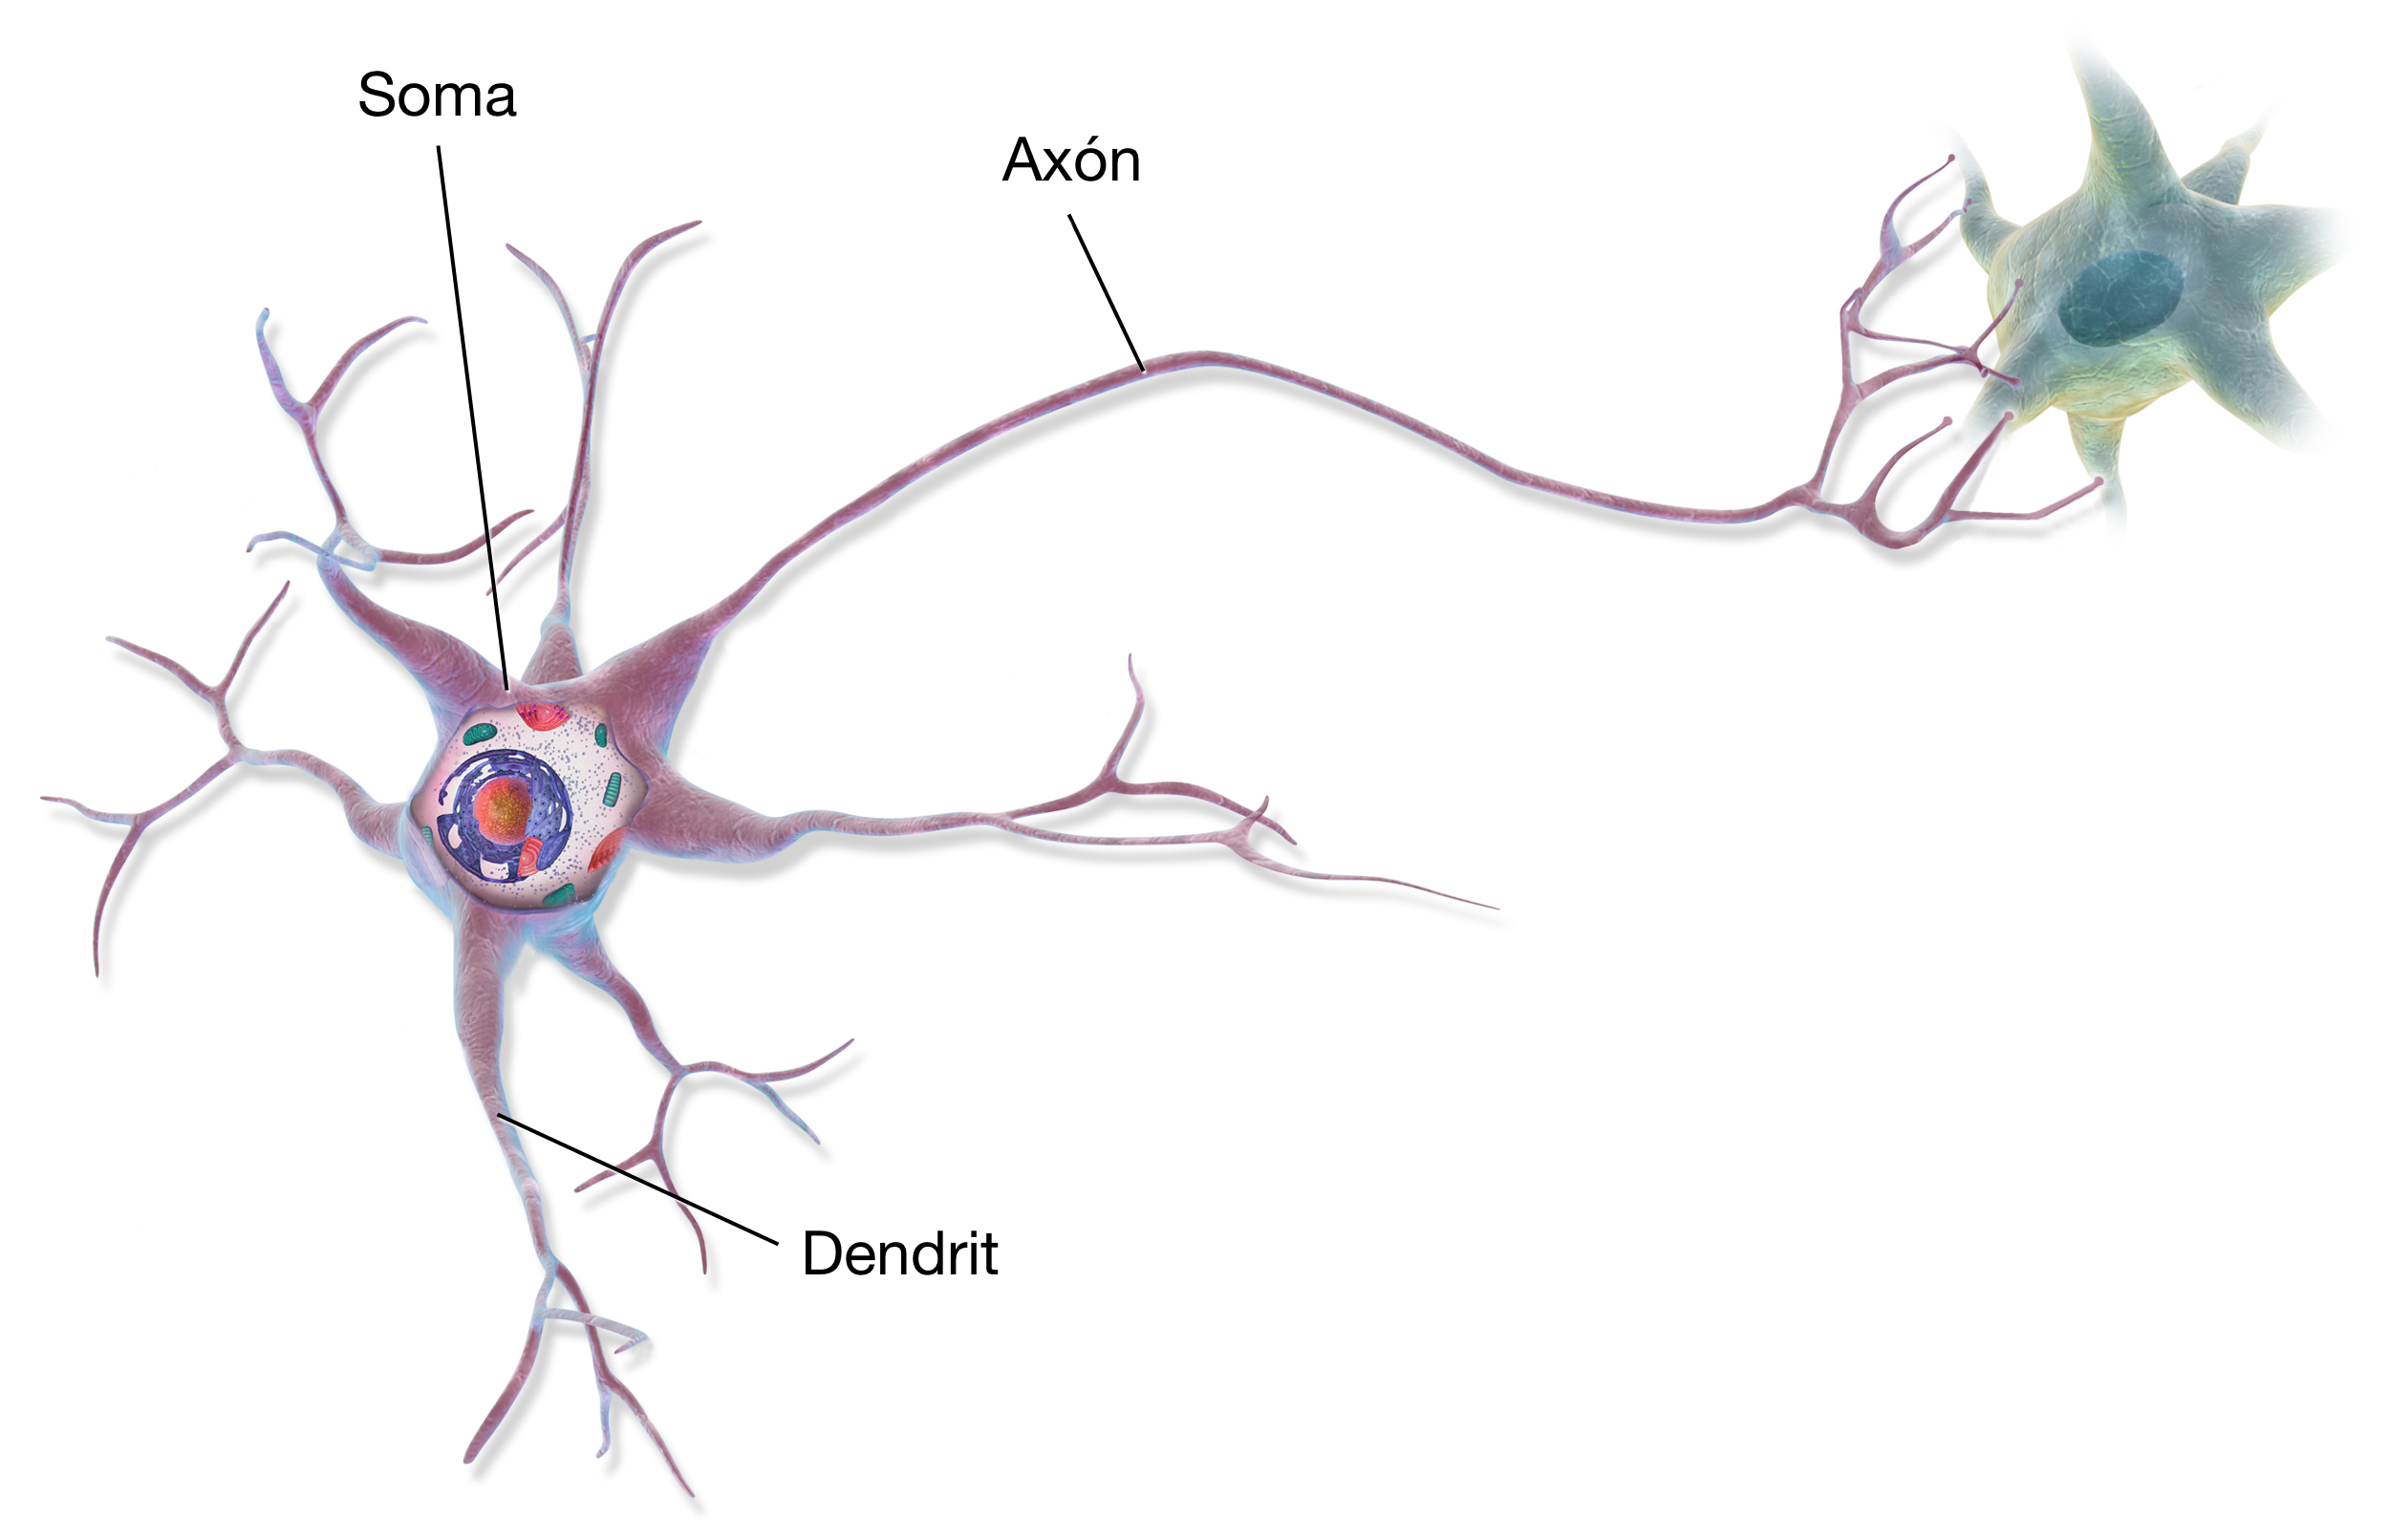
\includegraphics[width=0.8\textwidth]{BiologickyNeuron}
  \caption{Schéma biologického neurónu}
  \label{fig:BiologickyNeuron}
\end{figure}

\subsection{Neurotransmisia}

Neuróny medzi sebou komunikujú chemickým procesom, ktorý sa odohráva v medzere medzi neurónmi, v \emph{synapse}. Presynaptický neurón vylúči z konca axónu chemický mediátor, nazývaný \emph{neurotransmiter}, a ten sa naviaže na dendrit postsynapticého neurónu.

Množstvo vylúčeného mediátora priamo ovplyvňuje správanie postsynaptického neurónu. Ak \emph{súhrnný výsledok} prijatých neurotransmiterov presiahne istý \emph{prah}, neurón vygeneruje \emph{akčný potenciál}, ktorý zapríčiní vylúčenie mediátorov na axóne. Signál sa tak prenesie na ďalšie neuróny.

Poznáme dva typy mediátorov, \emph{excitačné} a \emph{inhibičné}. Excitačné mediátory zvyšujú šancu, že postsynaptický neurón bude aktívny. Naopak inhibičný mediátor znižuje aktivitu a tým klesá súhrnný výsledok, čo môže zapríčiniť neaktivitu postsynaptického neurónu.

\section{Umelý neurón}

Abstrahovaním funkcií biologického neurónu dostaneme umelý neurón, ktorý si zachováva výpočtové vlastnosti a zanedbáva nezaujímavé vlastnosti ako napr. metabolizmus. Schématický popis umelého neurónu je možné vidieť na obrázku \ref{fig:UmelyNeuron}.

\begin{figure}[H]
  \centering
  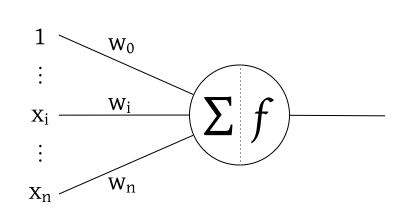
\includegraphics[width=7cm]{UmelyNeuron}
  \caption{Schéma umelého neurónu}
  \label{fig:UmelyNeuron}
\end{figure}

\subsection{Váhový vektor}

Neurón obsahuje niekoľko vstupov, ktoré nadobúdajú reálne hodnoty a predstavujú hodnoty, ktoré neurón chce spracovať:
\[
\mathbf{x} = (x_0, x_1, x_2, \ldots, x_n); \mathbf{x} \in \mathbb{R}^{n+1}
\]
Každý z týchto vstupov má svoju vlastnú váhu, ktorá odpovedá sile spojenia medzi neurónmi:
\[
\mathbf{w} = (w_0, w_1, w_2, \ldots, w_n); \mathbf{w} \in \mathbb{R}^{n+1}
\]
Ak je hodnota váhy kladná, hovoríme o excitačnom spojení. Ak je hodnota záporná, tak o inhibičnom. Nulová váha vyjadruje neexistujúce spojenie medzi neurónmi.

Sila signálu pre jeden vstup teda závisí na veľkosti vstupu ako aj na váhe spojenia:
\begin{eqnarray}
y_i = x_i \times w_i
\end{eqnarray}

Nultý člen oboch vektorov slúži ako špeciálna hodnota pre neurón, tzv. \emph{bias}. Vstup $x_0$ je fixne nastavený na hodnotu $1$ a váha $w_0$ nadobúda rôzne hodnoty. Úlohou biasu je škálovať ostatné vstupy.

\subsection{Sumačná funkcia}

Integrácia signálu je vykonaná sčítaním všetkých váhovaných vstupov dokopy\footnote{Akoby sa zabúdalo na to, že topológia dentritu je hierarchická.}, teda lineárna kombinácia vstupov a váh:
\begin{eqnarray}
y = \sum_{i=1}^{n} w_i x_i
\end{eqnarray}

Ak si zvolíme vektorovú reprezentáciu vstupných hodnôt a váh, tak integráciu môžeme vyjadriť ako skalárny súčin týchto vektorov:
\begin{eqnarray}
y = w \cdot x
\end{eqnarray}

\subsection{Prenosová funkcia}

Prenosová funkcia, často nazývaná aj aktivačná funkcia, má z hľadiska spracovania informácie dôležité postavenie. Jej úlohou je vyhodnotenie integrovaného signálu a propagácia do ďalších neurónov. Existuje viacero funkcií, ktoré sa používajú s väčšou, či menšou úspešnosťou.

\subsubsection{Funkcia identity}

Najjednoduchšou prenosovou funkciou je identita, teda neurón pošle ďalej iba nezmenený integrovaný signál:
\begin{eqnarray}
  f(y) = y
\end{eqnarray}

Táto funkcia má veľkú nevýhodu -- počíta iba lineárnu transformáciu vstupov. Ak by sme teda poskladali sieť z vrstiev, ktoré by obsahovali iba takéto neuróny, na výstupe by sme opäť dostali lineárnu transformáciu. A tú vieme vypočítať aj jednou vrstvou.

\begin{figure}[H]
  \centering
  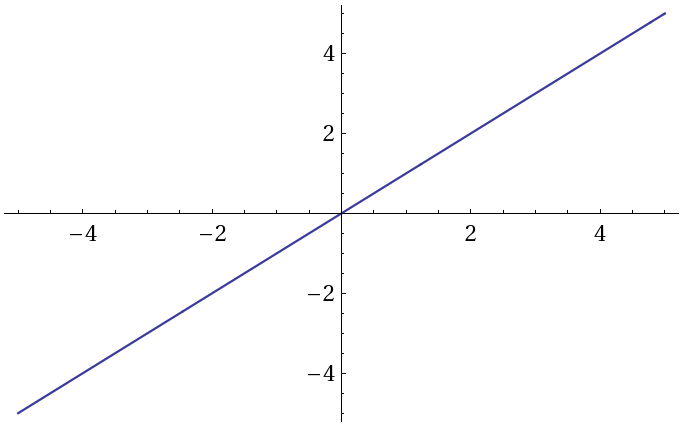
\includegraphics[width=7cm]{FunkciaIdentity}
  \caption{Funkcia identity}
  \label{fig:Identita}
\end{figure}

\subsubsection{Sigmoidálna funkcia}

Na vyriešenie problému s lineárnosťou výstupu sa začala používať nelineárna prenosová funkcia. Vhodným kandidátom bola jednoduchá sigmoidálna funkcia:
\begin{eqnarray}
  f(y) = \sigma(y) = \frac{1}{1 + e^{-y}}
\end{eqnarray}

\begin{figure}[H]
  \centering
  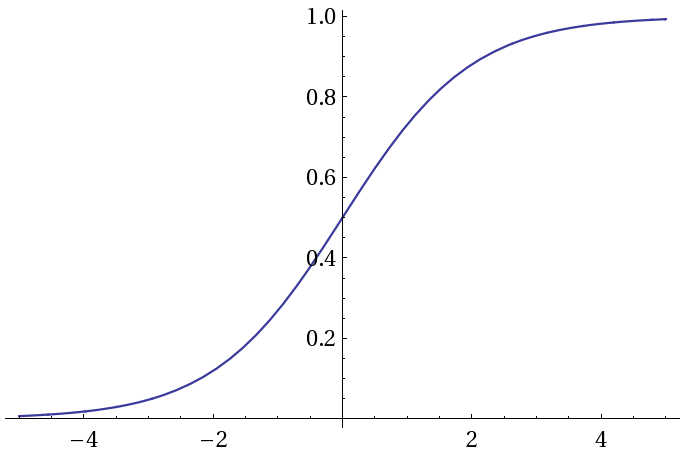
\includegraphics[width=7cm]{SigmoidalnaFunkcia}
  \caption{Sigmoidálna funkcia}
  \label{fig:SigmoidalnaFunkcia}
\end{figure}

Táto prenosová funkcia sa dlhú dobu používala ako štandard, ktorý poskytoval uspokojivé výsledky. Miernou nevýhodou tejto funkcie je jej derivácia, ktorá pri veľmi vysokých a veľmi nízkych hodnotách sa blíži k nule, čo spomaľuje učenie.

\subsubsection{Softplus funkcia}
Neurón používajúci \emph{softplus} prenosovú funkciu má veľmi zaujímavé správanie -- simuluje výpočet nekonečného počtu sigmoidálnych neurónov.\autocite{Nair2010}

Všetky kópie zdieľajú váhy, avšak každý neurón má mierne posunutý prah aktivácie o istú konštantu. Ak sú tieto konštanty rovné $-0{,}5, -1{,}5, -2{,}5,$ atď., tak výsledný súčet sa dá aproximovať uzavretou formou:
\begin{eqnarray}
  f(y) = \sum_{i=1}^{\infty}\sigma(y - i + 0{,}5) \approx \log_e(1 + e^y)
\end{eqnarray}

\begin{figure}[H]
  \centering
  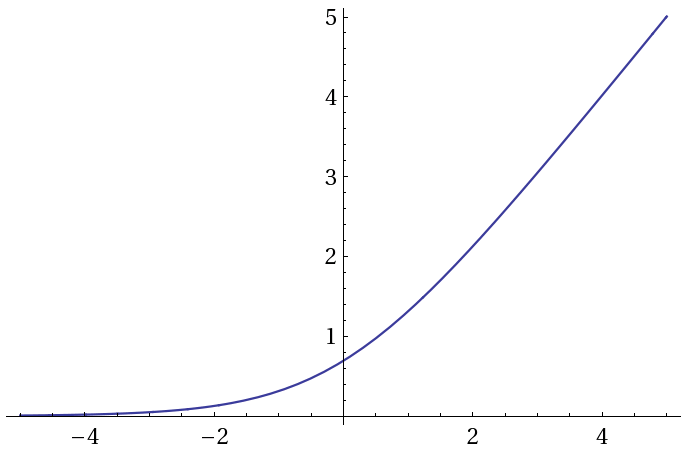
\includegraphics[width=7cm]{SoftplusFunkcia}
  \caption{Softplus funkcia}
  \label{fig:SoftplusFunkcia}
\end{figure}

Hoci má \emph{softplus} aktivačná funkcia veľmi zaujímavé vlastnosti, vysoká výpočtová náročnosť znemožňuje jej použitie v praxi.

\subsubsection{Funkcia max}

Pre softplus funkciu existuje aproximácia, ktorá si zachováva vynikajúce vlastnosti, avšak je výpočtovo nenáročná. Definovaná je nasledovne:
\begin{eqnarray}
f(y) = \max(0, y) =
\begin{cases}
0, & y \le 0 \\
y, & y > 0
\end{cases}
\end{eqnarray}

Táto funkcia je až zarážajúco jednoduchá -- pre nulu a záporné hodnoty vracia nulu a pre kladné hodnoty vracia nezmenený vstup, t.j. funkcia vracia väčší prvok z dvojice $(0, x)$. Vďaka výpočtovej nenáročnosti je funkcia $\max(0,y)$ veľmi vhodnou prenosovou funkciou pre hlboké siete s miliónmi, či dokonca miliardami spojení.

\begin{figure}[H]
  \centering
  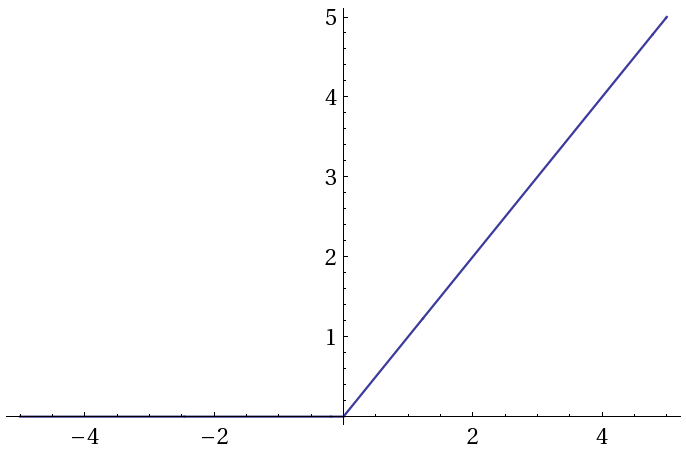
\includegraphics[width=7cm]{MaxFunkcia}
  \caption{Funckia $\max(0,y)$}
  \label{fig:MaxFunkcia}
\end{figure}

Ďalšou pozitívnou vlastnosťou tejto funkcie je jej derivácia definovaná nasledovne:
\begin{eqnarray}
f'(x) =
\begin{cases}
0, & x \le 0 \\
1, & x > 0
\end{cases}
\end{eqnarray}

Vidíme, že derivácia pre kladné hodnoty je vždy rovná jednej, čo znamená, že zmena váh bude vždy konštantná. Táto črta je obzvlášť pozitívna -- neurón netrpí tzv. problémom miznúceho gradientu chyby, ktorý komplikuje učenie hlbokých sietí. \autocite{Bengio1994}

Potenciálny problém nastáva až v druhom prípade, keď je aktivácia neurónu nulová, teda keď je vstup záporný alebo rovný nule. Keďže pri takýchto vstupoch je derivácia nulová, zmena váh nenastane. Tento fakt môže zapríčiniť tzv. \emph{smrť neurónu}, t.j. situáciu, kedy váhy neurónu produkujú nulovú aktiváciu, ktorá spätne nemá žiaden vplyv na zmenu jeho váh. V tomto prípade váhy ostávajú fixované bez možnosti akejkoľvek zmeny a neurón sa tak stáva zbytočným pretože nenastáva propagácia aktivácie. \autocite{Maas2013}

Nulová aktivácia sa na prvý pohľad môže zdať ako vážny problém, avšak opak je pravdou. Problém so stratou informácie sa vyrieši nasledovne: ak sa informácia prenesie aspoň cez jeden neurón vo vrstve, tak problém prestáva existovať. Tento jav  podporuje distribuované a riedke reprezentácie, čo činí takéto neuróny biologicky prijateľnými. \autocite{Glorot2011}

\section{Neurónové siete}

Spojením popísaných neurónov vytvoríme umelú \emph{neurónovú sieť}. Existuje mnoho spôsobov ako ich usporiadať aby vykonávali nejaký výpočet. Jednu z najpoužívanejších techník usporiadania neurónov predstavujú dopredné neurónové siete, ktorým sa budeme ďalej venovať.

\emph{Dopredné neurónové} siete nemajú spätnú väzbu, t.j. signál sa propaguje len jedným smerom cez vrstvy rôzneho typu. Každá vrstva zachytáva opakujúce sa pravidelnosti vo výstupoch predchádzajúcej vrstvy, čím vzniká hierarchická interakcia medzi neurónmi.

Hoci majú dopredné siete obmedzenú výpočtovú schopnosť kvôli chýbajúcej spätnej väzbe, stále ostávajú dobrou voľbou na mnoho problémov. Výborné výsledky podávajú najmä pri probléme klasifikácii vizuálnych vnemov, teda rozpoznávaní objektov na obrázkoch.

\subsubsection{Supervision}

\begin{figure}
  \centering
  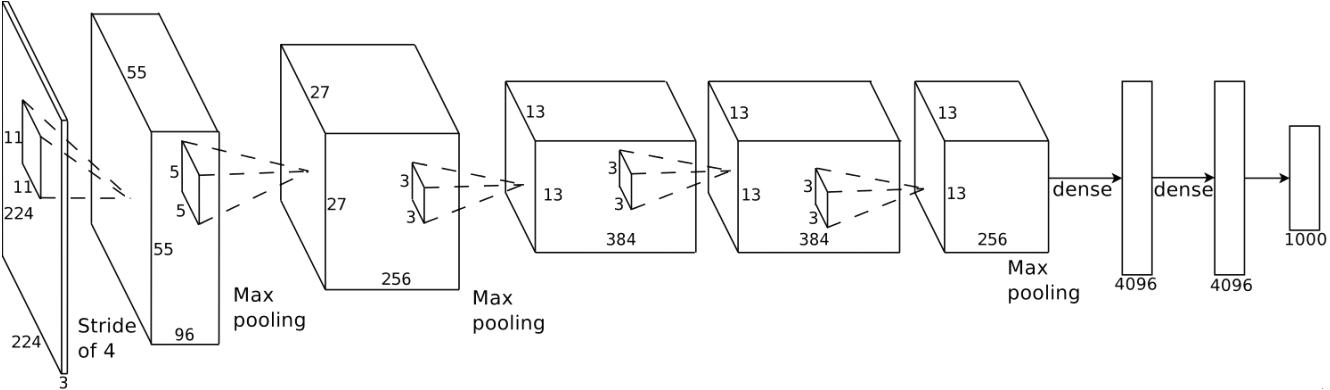
\includegraphics[width=\textwidth]{Supervision}
  \caption{Architektúra neurónovej siete Supervision}
  \label{fig:Supervision}
\end{figure}

Vynikajúce výsledky v rozpoznávaní objektov dosiahla konvolučná neurónová sieť \emph{Supervision}\autocite{Krizhevsky2012}, ktorej architektúra je zobrazená na obrázku \ref{fig:Supervision}. Táto sieť je tvorená z nasledujúcich typov vrstiev: vstupná vrstva, konvolučná vrstva, max-pooling vrstva, úplne prepojená vrstva a výstupná vrstva. Každú si teraz stručne popíšeme.

\subsection{Vstupná vrstva}

Vstupná vrstva neurónovej siete reprezentuje \emph{senzorické neuróny}, ktoré signalizujú prítomnosť (zvyčajne) externej informácie.

V biologických systémoch to je napr. \emph{sietnica} v oku, kde neuróny detegujú prítomnosť fotónov istej vlnovej dĺžky. V umelých systémoch je sietnica reprezentovaná neurónmi, ktoré si zachovávajú dvojrozmernú štruktúru vizuálneho vnemu.

Hodnoty vstupných neurónov reprezentujú intenzitu farby v danom bode obrazu. Ak máme iba čierno-biely vstup, tak neurón vyjadruje jas bodu -- nízke hodnoty vyjadrujú nedostatok informácie (málo svetla), a opačne. Pri farebných obrázkoch to platí pre každý kanál zvlášť.

Podstatnou vlastnosťou vstupnej vrstvy by mala byť normalizácia vstupných hodnôt, t.j. hodnoty by mali spadať do istého rozsahu. V biologických systémoch túto úlohu zohráva \emph{zrenica}, ktorá zamedzuje prílišnému príjmu svetla na sietnicu.

\subsection{Konvolučná vrstva}

Konvolučná vrstva\autocite{LeCunn1998} je biologicky inšpirovaná výskumom vizuálneho kortexu cicavcov, kde boli identifikované neuróny, ktoré sú vysoko citlivé na malé výseky vizuálneho vstupu. \emph{Receptívne polia}, ako sa tieto oblasti nazývajú, pokrývajú celé vizuálne pole a sú špecializované na detekciu vzorov zvyčajne podobných hranám.\autocite{Hubel1968}

Konektivita týchto neurónov je simulovaná procesom \emph{konvolúcie}. Konvolúcia (viď. obr.~\ref{fig:Konvolucia}) je matematická operácia, ktorá produkuje prekryv dvoch funkcií, v tomto prípade dvoch obrázkov. Prvý obrázok je výrez zo vstupnej vrstvy neurónovej siete a druhý obrázok je receptívne pole registrujúce nejakú črtu. Výsledkom prekryvu týchto obrázkov je hodnota, ktorá odpovedá odozve neurónu na daný stimul.

Výhodou konvolučnej vrstvy je zdieľanie parametrov -- váhy neurónu, ktorý detekuje istú črtu, sú použité na celý vizuálny vstup. Napr. na detekciu 45\degree{} hrany bude potrebný iba jeden špecializovaný neurón, ktorý bude použitý na celý vstup, nielen na vybranú oblasť.

\begin{figure}
  \centering
  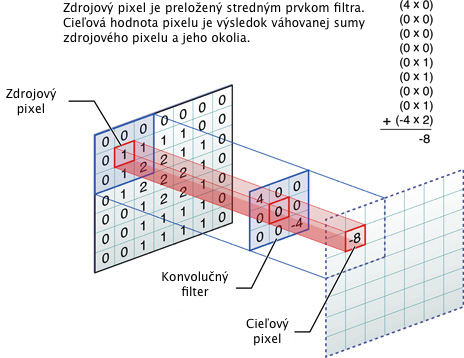
\includegraphics[width=10cm]{Konvolucia}
  \caption{Konvolúcia}
  \label{fig:Konvolucia}
\end{figure}

Konvolučná vrstva má niekoľko nastaviteľných parametrov, ktoré ovplyvňujú jej správanie a veľkosť výstupu:
\begin{enumerate}
  \item počet filtrov
  \item veľkosť filtra, napr. $3 \times 3$
  \item veľkosť kroku konvolúcie v oboch smeroch, napr. $1 \times 1$
\end{enumerate}

\subsection{Pooling vrstva}

Podobne ako konvolučná, tak aj pooling vrstva je biologicky inšpirovaná vizuálnym kortexom cicavcov. Bunky, ktoré sú modelované pooling vrstvou majú väčšie receptívne pole a sú lokálne invariantné na stimuly.

Pooling vrstva zvyčajne nasleduje za konvolučnou vrstvou a znižuje veľkosť vstupnej informácie procesom \emph{podvzorkovania}. Neurón v max-pooling vrstve propaguje iba salientné črty, ktoré konvolučná vrstva zachytila. Výstupom takejto vrstvy sú teda maximálne aktivácie z predchádzajúcej vrstvy. Výpočet závisí iba na vstupoch -- nepoužíva sa žiaden váhový vektor.

Rovnako ako konvolučná vrstva, tak aj pooling vrstva pracuje s výrezmi vstupov, ktoré sú parametrizované nasledujúcimi hodnotami:
\begin{enumerate}
  \item veľkosť okna, napr. $5 \times 5$
  \item veľkosť kroku v oboch smeroch, napr. $2 \times 2$
\end{enumerate}

\subsection{Úplne prepojená vrstva}

Úplne prepojená vrstva neobmedzuje konektivitu v žiadnom smere -- všetky neuróny v takejto vrstvy sú spojené meniteľnými váhami s každým neurónom z predchádzajúcej vrstvy. Kvôli tomuto je počet spojení vysoký, čím je učenie siete pomalšie.

\subsubsection{Regularizácia}

Pri veľkej vrstve zvykne dochádzať k situácii, kedy trénovacie dáta sú naučené príliš dobre. V takomto prípade neurónová sieť slabo generalizuje, čo sa prejaví ako zlé výsledky na testovacích dátach.

Možnosťou ako sa vyhnúť tomuto javu je použitie novej regularizačnej techniky, tzv. \emph{dropoutu}\autocite{Hinton2012}. Táto technika zabraňuje koadaptácii váh neurónov vnesením šumu do aktivácie neurónov.

Každý neurón v úplne prepojenej vrstve má pravdepodobnosť aktivácie rovnú ${p=0{,}5}$. To znamená, že pri každom trénovacom prípade používame iba polovicu neurónov a vždy inú sadu. Na dropout sa teda môžeme pozerať ako na trénovanie $2^n$ rôznych modelov zdieľajúcich váhy, pričom každý model je trénovaný len na jednom prípade.

\subsection{Výstupná vrstva} 

Neurónová sieť, ktorá je určená na klasifikáciu vnemov, zvyčajne produkuje pravdepodobnosť do akej kategórie patrí nejaký stimul. Na výpočet týchto pravdepodobností sa používa tzv. \emph{softmax} funkcia definovaná nasledovne:

\begin{eqnarray}
p_j = \frac{e^{y_j}}{\sum\limits_{k=1}^n e^{y_k}}
\end{eqnarray}

Index maximálnej hodnoty z vektoru pravdepodobností $p$ nám udáva kategóriu, ktorá produkuje najvyššiu mieru istoty pre nejaký stimul.

% BREAKING BAD

\chapter{Interaktívne experimentovanie}

Človek sa učí na základe skúseností s prostredím, ktoré mu poskytuje odozvu na jeho akcie. Ak je táto odozva nedostatočná, učenie môže prebiehať iba ťažko. Nástroj, ktorý umožňuje jednoduché použitie neurónových sietí, musí poskytovať prostredie, kde je možné pocítiť dôsledok vykonaných akcií okamžite.

\section{Súčasné riešenia}

Väčšina nástrojov, ktoré poskytujú funkcionalitu neurónových sietí, neumožňuje \emph{aktívne} spoznávať princíp ich fungovania. Tieto nástroje sú určené pre ľudí, ktorí ich používajú na riešenie špecifických problémov, nie na pochopenie ich správania. Príkladom takého nástroja môže byť Caffe\footnote{\url{http://caffe.berkeleyvision.org/}}, ConvNetJS\footnote{\url{http://cs.stanford.edu/people/karpathy/convnetjs/}}, Cuda-ConvNet\footnote{\url{https://code.google.com/p/cuda-convnet/}}, EBLearn\footnote{\url{http://eblearn.sourceforge.net/}}, Pylearn2\footnote{\url{http://deeplearning.net/software/pylearn2/}}, Torch\footnote{\url{http://torch.ch/}} a ďalšie.

Všetky tieto nástroje obsahujú možnosť naprogramovania želanej neurónovej siete použitím rôznych programovacích jazykov. Od programátora sa teda vyžaduje len absolútne minimum -- vedieť programovať a rozumieť neurónovým sieťam.

\subsection{Špecializované jazyky}

Isté nástroje poskytujú veľmi šikovné riešenie pre prvý problém. Keďže učenie neurónovej siete vyžaduje len popis architektúry a niekoľko ďalších parametrov, ovládať všeobecný programovací jazyk je zbytočné.

Riešením tohoto problému sú popisné jazyky, ktoré špecifikujú iba potrebné parametre pre vytvorenie a učenie neurónovej siete. Ako takýto jazyk vyzerá, je možné vidieť na nasledovnej ukážke:

\begin{lstlisting}[multicols=2]
name: "network"
input: "data"
input_dim: 64
input_dim: 1
input_dim: 28
input_dim: 28

layers {
  name: "conv"
  type: CONVOLUTION
  bottom: "data"
  top: "conv"
  convolution_param {
    num_output: 9
    kernel_size: 5
    stride: 1
  }
}

layers {
  name: "relu"
  type: RELU
  bottom: "conv"
  top: "pool"
}

layers {
  name: "pool"
  type: POOLING
  bottom: "relu"
  top: "pool"
  pooling_param {
    pool: MAX
    kernel_size: 2
    stride: 2
  }
}

layers {
  name: "ip"
  type: INNER_PRODUCT
  bottom: "pool"
  top: "ip"
  inner_product_param {
    num_output: 10
  }
}

layers {
  name: "prob"
  type: SOFTMAX
  bottom: "ip"
  top: "prob"
}
\end{lstlisting}

Formáty, ktoré sa používajú na tento druh popisu zahŕňajú \emph{XML}\autocite{Beran2008}, \emph{JSON}\footnote{\url{http://cs.stanford.edu/people/karpathy/convnetjs/}} a \emph{Protocol Buffers}\footnote{\url{http://caffe.berkeleyvision.org/}}. Ako reprezentácia väčšiny programovacích jazykov, aj tieto formáty sú primárne určené na \emph{uchovávanie obsahu}, nie na priamu interakciu s nimi.

\subsection{Vizualizácia}

Väčšina spomínaných nástrojov ponúka možnosť čiastočnej vizualizácie neurónových sietí. Tieto vizualizácie pomáhajú pochopiť správanie sa siete.

Najpoužívanejšou zobrazovacou technikou je monitorovanie priebehu učenia v čase, viď. obrázok \ref{fig:ChybaUcenia}. Táto jednoduchá vizualizácia nám pomáha zistiť, či sa sieť skutočne učí. Veľkou pomôckou je aj pri rozhodovaní o tom, kedy treba zastaviť trénovanie. Ak by sme zastavili trénovanie neskoro, sieť by mala výborné výsledky na trénovacej množine, avšak na testovacích dátach by pohorela.

\begin{figure}
  \centering
  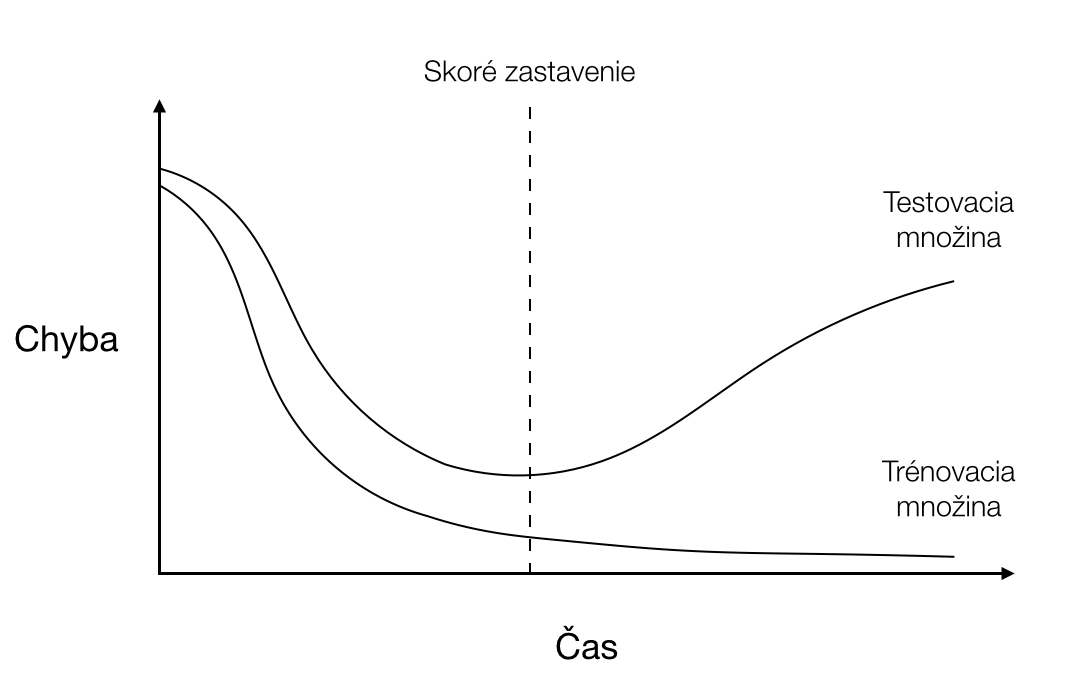
\includegraphics[width=10cm]{ChybaUcenia}
  \caption{Ukážka vizualizácie trénovania neurónovej siete}
  \label{fig:ChybaUcenia}
\end{figure}

Ďalším štandardom vo vizualizácii neurónových sietí je možnosť zobrazenia filtrov, resp. váh neuronálnych spojení. Na obrázku \ref{fig:SupervisionFiltre} sú zobrazené filtre z prvej vrstvy siete Supervision.\autocite{Krizhevsky2012} Podrobným skúmaním filtrov z celej siete sme schopní zistiť o vnútorných reprezentáciách systému omnoho viac.\autocite{Zeiler2013}

\begin{figure}
  \centering
  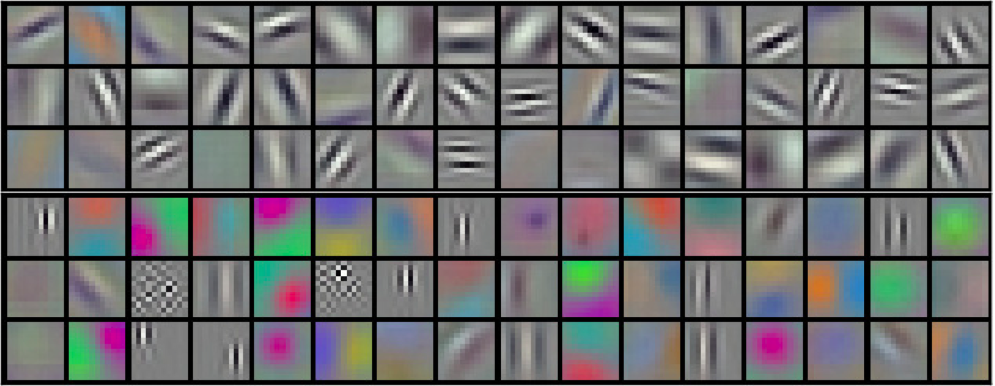
\includegraphics[width=10cm]{SupervisionFiltre}
  \caption{Vizualizácia filtrov z prvej vrstvy siete Supervision}
  \label{fig:SupervisionFiltre}
\end{figure}

% Tu sa začína sranda. %

\section{Navrhované riešenie}

Predpokladajme, že existuje lepšie riešenie ako tie, ktoré sme si doteraz popísali. Čím je iné? Čo by malo spĺňať aby mohli neurónové siete používať aj ľudia, ktorí nevedia programovať?

\subsection{Princípy}

V nasledujúcej časti si popíšeme princípy, ktoré sú esenciálne pre navrhované riešenie nástroja na interaktívne experimentovanie s neurónovými sieťami.

\subsubsection{Reprezentácie}

Jerome Brunner popísal tri stupne reprezentácií, ktoré používame pri vytváraní si nových koncepcií.\autocite{Bruner1966} Popíšeme si ich na príklade kvadratickej funkcie.
\begin{description}
  \item[Enaktívne reprezentácie] pozostávajú z akcií, ktoré môžeme vykonávať \emph{priamou manipuláciou} s objektami. Napr. dieťa hrajúce sa s kockami môže kvadratickú funkciu vyjadriť rozmiestnením kociek do štvorcovej formácie.
  \item[Ikonické reprezentácie] vyjadrujú \emph{vizuálne vlastnosti} konkrétnych situácií naučených v enaktívnej fáze. Napr. akýkoľvek obrázok štvorca alebo graf kvadratickej funkcie spadajú do tejto kategórie.
  \item[Symbolické reprezentácie] popisujú abstraktné informácie o naučených konceptoch cez \emph{dohodnuté symboly}. Kvadratická funkcia je symbolicky vyjadrená ako $a \times a$ alebo $a^2$, kde symboly popisujú entity a aj manipulácie s nimi.\footnote{Zaujímavosťou je fakt, že symbolické reprezentácie môžu vyjadrovať aj inštancie situácií, ktoré nemôžeme poňať v enaktívnej fáze, napr. \uv{štvorec so zápornou dĺžkou strany}.}
\end{description}

Ktoré reprezentácie treba použiť aby bol zabezpečený čo najlepší prenos a uchovanie informácie? Enaktívne, ikonické alebo symbolické? Ideálne všetky naraz. Použitím všetkých získava človek intuíciu o tom, aké vzťahy existujú medzi jednotlivými časťami systému na rôznych úrovniach opisu.

\subsubsection{Vizuálne programovanie}

Ako vyzerá prostredie, ktoré by poskytovalo použitie všetkých troch druhov reprezentácií? Textový editor, kde napíšeme zdrojový kód neurónovej siete, to určite nie je.

\emph{Vizuálne programovanie} (obr. \ref{fig:QuartzComposer}) sa ponúka ako vhodná paradigma, ktorá je používaná s väčšou, či menšou úspešnosťou v rôznych oblastiach návrhu komplexných systémov.

\begin{figure}[b]
  \centering
  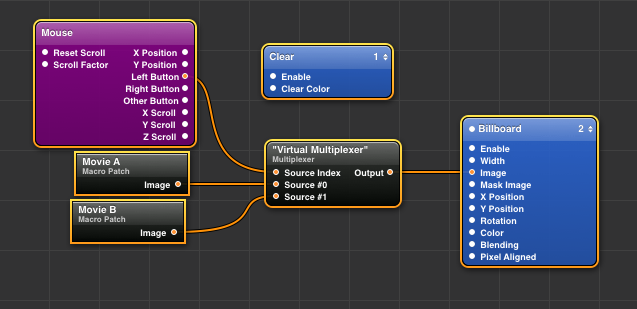
\includegraphics[width=0.8\textwidth]{QuartzComposer}
  \caption{Ukážka vizuálneho programovania}
  \label{fig:QuartzComposer}
\end{figure}

Paradigma vizuálneho programovania používa \emph{plátno}, na ktorom sú umiestnené \emph{objekty}. Každý objekt obsahuje vstupy, ktoré transformuje na výstupy. Tieto výstupné hodnoty sú potom použité ako vstupné hodnoty do ďalšej transformácie.

Každý objekt predstavuje transformáciu dát, ktoré prúdia po spojeniach medzi nimi. Táto vizuálna forma je teda veľmi vhodná na zobrazovanie architektúry neurónových sietí a poslúži nám ako základ pre ďalšie úpravy.

\subsubsection{Dáta $\gg$ Model}

Veľmi dôležitá skutočnosť, na ktorú sa často zabúda je, že \emph{dáta sú dôležitejšie ako model}. Aj ten najlepší model na svete je bezvýznamný bez dát, ktoré by mohol modelovať.

Problémom vizuálneho programovania je absencia akýchkoľvek dát. Objekty na ploche reprezentujú iba transformácie, avšak samotné dáta nie sú zobrazené. Vizuálna paradigma je týmto redukovaná na slepú manipuláciu so symbolmi, čo silne obmedzuje použitie tohto prístupu.

Najjednoduchším riešením tohto obmedzenia je \emph{zobrazenie transformovaných dát}. Ak zobrazíme dáta v každom kroku transformácie, používateľovi pomáhame pochopiť jednotlivé časti systému. Experimentovaním si používateľ osvojí časti systému, čím sa mu otvára možnosť k pochopeniu neurónovej siete ako celku.\autocite{Victor2013}

\subsection{Popis riešenia}

\subsubsection{Problém}

Zaveďme si ilustratívny problém, ktorý chceme vyriešiť. V oblasti strojového učenia to zvyčajne býva \emph{MNIST} -- problém rozpoznávania rukou písaných číslic.\autocite{LeCunn1998} Tento dataset je relatívne malý a pozostáva zo $60{~}000$ trénovacích a $10{~}000$ testovacích príkladov.

Každý jeden vstupný vzor je $28 \times 28$ pixelový obrázok v odtieňoch šedej. Požadovaným výstupom má byť zaradenie obrázku do správnej kategórie. Vybrané ukážky z dátovej množiny je možno vidieť na obrázku~\ref{fig:MNIST}.

\begin{figure}[b]
  \centering
  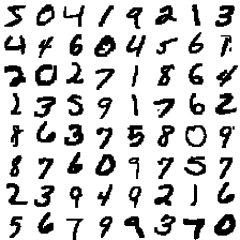
\includegraphics[width=5cm]{MNIST}
  \caption{Ukážka príkladov z MNIST}
  \label{fig:MNIST}
\end{figure}

\subsubsection{Riešenie}

Problém, ktorý chceme vyriešiť, je tvorený zo 70 tisíc menších problémov. Redukujme si teda náš problém a teda aj dátovú množinu na jeden príklad, na ktorý sa budeme sústrediť.

Vložíme na plochu jeden obrázok, ktorý prostredie automaticky rozpozná ako dátový zdroj:

\begin{figure}[H]
  \centering
  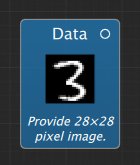
\includegraphics[scale=0.57]{UI/DataSource}
  \caption{Dátový zdroj}
\end{figure}

Tento objekt má tri vlastnosti, ktoré definujú jeho existenciu na ploche. Prvou vlastnosťou, ktorú môžeme vidieť, je jeho \emph{vizuál}. Objekt zapuzdruje vnútorné dáta a farbou vyjadruje svoj typ.

Ďalšou vlastnosťou je \emph{symbolický popis}. Okrem prednastaveného mena máme k dispozícii aj textový opis dát, ktorý stručne charakterizuje zobrazené dáta. 

Poslednou vlastnosťou je \emph{priama manipulácia}. Objekt môžeme ťahaním premiestňovať po ploche, čím mu môžeme nastaviť polohu, ktorá nám vyhovuje. Rovnako mu môžeme zmeniť aj jeho ďalšie vlastnosti.

\bigskip

Priama manipulácia s objektom zahŕňa aj zmenu prednastaveného mena:

\begin{figure}[H]
  \centering
  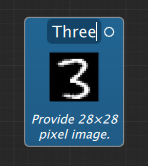
\includegraphics[scale=0.57]{UI/DataSourceRename}
  \caption{Premenovanie dátového zdroja}
\end{figure}

Premenovanie objektu nám umožňuje priradiť mu deskriptor, ktorý viac vyhovuje našim požiadavkám. V tomto prípade sme premenovali dátový zdroj na meno vyjadrujúce popis dát, ktoré ponúka, teda číslo \uv{tri}.

\bigskip

Nenápadný kruh na pravej strane komponentu predstavuje výstupnú hodnotu objektu. V tomto prípade sa jedná o vnútorné dáta, ktoré objekt poskytuje, t.j. obrázok čísla tri.

Aby sme mohli použiť tieto dáta v nejakej transformácii, musíme tento komponent spojiť s iným komponentom. V súlade s koncepciou priamej manipulácie je tento kruh \emph{ťahateľný}. Ťahaním sa nám zobrazí \emph{konektor}, ktorý spája objekt s voľným uzlom, ktorý pripneme k inému objektu:

\begin{figure}[H]
  \centering
  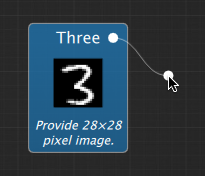
\includegraphics[scale=0.57]{UI/DataSourceDragConnector}
  \caption{Ťahanie výstupného konektoru dátového zdroja}
\end{figure}

Nastal však problém. Na ploche existuje iba jeden objekt a ten chceme na nejaký napojiť -- nemáme žiadne ďalšie objekty, ktoré by sme mohli použiť. Potrebujeme vytvoriť nový objekt, ktorý použijeme.

Konektor pustíme na prázdnu plochu. Zobrazí sa nám \emph{ponuka}, z ktorej si môžeme vybrať komponent, ktorý nám vyhovuje:

\begin{figure}[H]
  \centering
  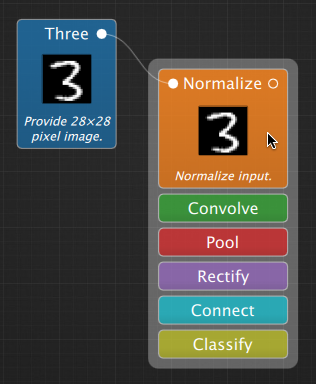
\includegraphics[scale=0.57]{UI/NormalizePreview}
  \caption{Ponuka transformácií s okamžitým náhľadom}
\end{figure}

Ponuka obsahuje všetky transformácie, ktoré môžeme pridať na plochu. Vidíme, že názvy transformácií používajú \emph{slovesný tvar}. To zdôrazňuje fakt, že komponenty vykonávajú istú \emph{funckiu}. Tento prístup je vhodnejší ako názov, ktorý implikuje iba pasívnu úlohu, napr. \uv{normalizácia} verzus \uv{normalizovať} alebo \uv{normalizuj}.

Dôležitou vlastnosťou ponuky komponentov je \emph{okamžitý náhľad}. Ten môžeme vidieť na príklade normalizačnej transformácie. Vďaka vizuálnemu zobrazeniu a textovému popisu vieme, čo máme očakávať od danej transformácie. Vďaka tejto vlastnosti sa môžeme vyhnúť zbytočnej manipulácii s objektami na ploche.

Máme predvolenú normalizačnú vrstvu, ktorá nám upraví rozsah vstupných hodnôt na požadované rozpätie. Túto úlohu zvyčajne vykonáva \emph{vstupná vrstva} siete, avšak názov \uv{vstupná vrstva} nám nepovie nič o jej funkcii.

\bigskip

Zdá sa však, že výstup z dátového zdroja a výstup z normalizačnej transformácie sú úplne rovnaké -- akoby transformácia nemala žiaden vplyv na dáta. A to je aj pravda. Dáta, ktoré používame, sú poskytnuté v normalizovanej forme -- ďalšia normalizácia nebude mať žiaden efekt. Okamžitý náhľad nám pomohol zbaviť sa nepotrebnej transformácie ešte predtým ako sme ju vôbec použili.

\bigskip

Zvoľme teda zaujímavejšiu vrstvu, ktorá nám pomôže pri našom probléme rozpoznávania číslic. Konvolučná vrstva je vhodnou voľbou:

\begin{figure}[H]
  \centering
  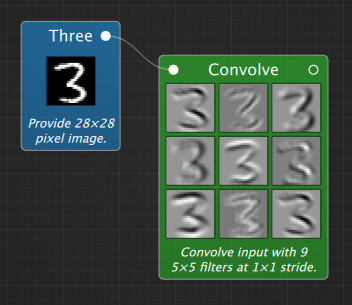
\includegraphics[scale=0.57]{UI/Convolve}
  \caption{Konvolučná vrstva}
\end{figure}

Konvolučná vrstva produkuje viacero výstupov a každý jeden z nich môžeme \emph{vidieť}. Vďaka textovému popisu vieme \emph{povedať} čo daná transformácia vykonáva. Avšak až vďaka priamej manipulácii si môžeme začať budovať koncepcie o tom ako táto transformácia skutočne funguje.

\bigskip

Pri prechádzaní ponad výstup konvolučnej vrstvy sa nám na dátovej vrstve zobrazí výrez obrázku, ktorý bol použitý na vypočítanie hodnoty danej aktivácie:

\begin{figure}[H]
  \centering
  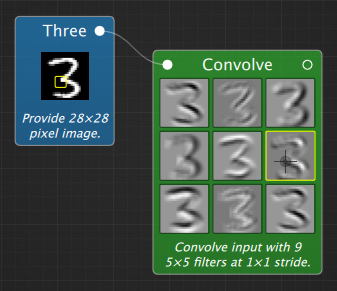
\includegraphics[scale=0.57]{UI/ConvolveHover}
  \caption{Spojené reprezentácie}
\end{figure}

Z tejto interakcie je nám jasné, že každá jedna aktivácia na konvolučnej vrstve je asociovaná s istou časťou zdrojového obrázka. Avšak prečo transformácia produkuje 9 výstupov? Na túto otázku nám čiastočne odpovedá textový popis, v ktorom sa spomína \uv{9 filtrov veľkosti $5 \times 5$}. Vidíme, že počet výstupov bude závislý od počtu filtrov, ktoré použijeme. Ale čo sú filtre? Navyše odkiaľ sa zobrali takéto parametre? Žiaden z nich sme nenastavovali.

Kliknutím na textový opis odkryjeme dôležitú časť tejto transformácie -- skryté parametre:

\begin{figure}[H]
  \centering
  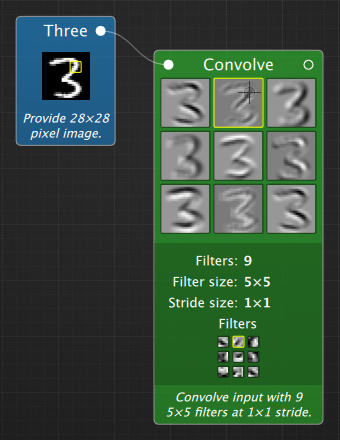
\includegraphics[scale=0.57]{UI/ConvolveExtended}
  \caption{Nastaviteľné parametre konvolučnej vrstvy}
\end{figure}

Prvé čo si všimneme sú vizuálne reprezentácie filtrov, ktorých je skutočne deväť. Ďalej vidíme tri parametre, ktoré ovplyvňujú správanie transformácie. Tieto parametre sú meniteľné ťahaním -- chytíme číselný parameter a potiahnutím doľava alebo doprava meníme jeho hodnotu. Všetky zmeny sa prejavia okamžite, čím sa pocit slepej manipulácie so symbolmi úplne rozplynie.

\bigskip

Ukážme si takúto zmenu na príklade počtu filtrov. Miernym potiahnutím doľava znížime hodnotu parametra z 9 na 8. Táto zmena sa prejaví na ďalších troch rôznych miestach -- počet výstupov transformácie, počet filtrov a nakoniec aj v textovom popise:

\begin{figure}[H]
  \centering
  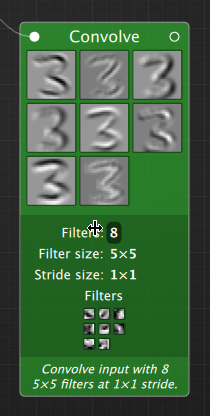
\includegraphics[scale=0.57]{UI/ConvolveChangeFilters}
  \caption{Zmena počtu filtrov konvolučnej vrstvy}
\end{figure}

Táto zmena je celkom zjavná a očakávaná -- počet filtrov je vo vzájomnom vzťahu s počtom výstupov. Čo však ďalšie parametre? Skúsme zmeniť veľkosť kroku z hodnoty $1 \times 1$ na $2 \times 2$. Táto zmena má celkom neočakávané správanie:

\begin{figure}[H]
  \centering
  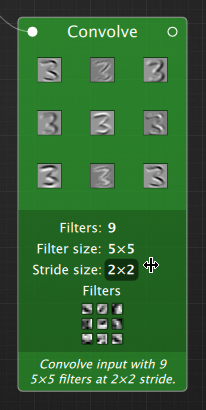
\includegraphics[scale=0.57]{UI/ConvolveChangeStride}
  \caption{Zmena kroku konvolučnej operácie}
\end{figure}

Veľkosti jednotlivých výstupov sa zmenšili na polovicu. Po vyskúšaní niekoľkých ďalších hodnôt zistíme, že veľkosť kroku konvolúcie funguje ako škálovací operátor, ktorý redukuje veľkosť výstupov. Symbol \uv{krok konvolúcie} žiadne takéto správanie neobjasňuje. Interaktívna manipulácia parametrov nám pomohla rýchlejšie pochopiť skryté súvislosti, ktoré sa len ťažko vysvetľujú matematickým formalizmami, či zdrojovým kódom nejakého počítačového programu.

\bigskip

Pridajme ďalšiu transformáciu, ktorá bude spracúvať výstup z konvolučnej vrstvy:

\begin{figure}[H]
  \centering
  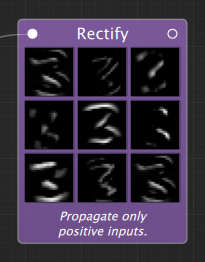
\includegraphics[scale=0.57]{UI/Rectify}
  \caption{Jednoduchá transformácia}
\end{figure}

Transformácia rectify funguje ako prechodová funkcia neurónu. Táto inštancia prechodovej funkcie ignoruje záporné aktivácie z predchádzajúcej vrstvy a posiela ďalej iba kladné hodnoty. Keďže táto transformácia nemá žiadne nastaviteľné parametre dá sa jej venovať iba málo.

\bigskip

Pridajme pooling vrstvu, ktorá združuje aktivácie z predchádzajúcej vrstvy a berie z nich iba maximálne hodnoty, tzv. \emph{max-pooling} vrstva:

\begin{figure}[H]
  \centering
  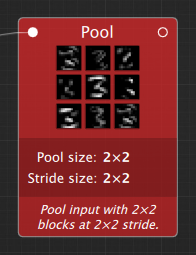
\includegraphics[scale=0.57]{UI/Pool}
  \caption{Max-pooling vrstva}
\end{figure}

Táto transformácia je veľmi podobná konvolučnej vrstve, avšak akoby jej funkcia bola  o niečo obmedzená. Pooling vrstva nepoužíva žiadne filtre a zvyšné dva parametre sa správajú rovnako ako parametre konvolučnej vrstvy, čo môžeme vidieť na príklade spojených reprezentácií:

\begin{figure}[H]
  \centering
  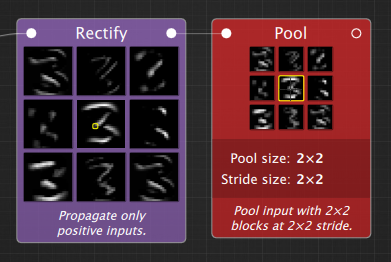
\includegraphics[scale=0.57]{UI/PoolHover}
  \caption{Spojené reprezentácie na max-pooling vrstve}
\end{figure}

Zdá sa, že pooling vrstva iba zmenšuje výstup z rectify vrstvy. Možno teda vôbec nezáleží na ich poradí\dots Avšak skúsme pokračovať pridaním plne prepojenej vrstvy. Tej nastavíme veľkosť na desať, teda počet tried, do ktorých chceme zaradiť naše dáta:

\begin{figure}[H]
  \centering
  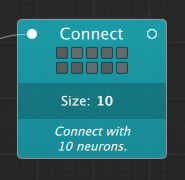
\includegraphics[scale=0.57]{UI/Connect}
  \caption{Úplne prepojená vrstva}
\end{figure}

Vidíme, že aktivácie na tejto vrstve sú takmer totožné a všetky sa držia približne v strednej hodnote. Avšak táto vrstva je iba medzistupňom k tomu aby sme skutočne videli to, čo si neurónová sieť \emph{myslí} o danom vstupe. Pridajme teda poslednú vrstvu, ktorá nám túto informáciu sprostredkuje:

\begin{figure}[H]
  \centering
  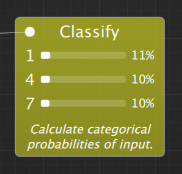
\includegraphics[scale=0.57]{UI/Classify}
  \caption{Klasifikačná vrstva}
\end{figure}

Klasifikačná vrstva nám zobrazuje tri najpravdepodobnejšie tipy vrátane miery istoty, ktorá je vyjadrená vizuálne a aj číselne. Všetky triedy majú mieru istoty okolo 10\%, čo nám hovorí, že neurónová sieť si svojimi tipmi nie je vôbec istá. Toto je dobré znamenie, pretože neurónová sieť ešte nevie nič o rozpoznávaní číslic, takže by nemala preferovať žiadnu triedu.

Posledná vec, ktorá nám ostáva urobiť, je natrénovať sieť, aby sa naučila rozpoznávať číslice.

\bigskip

\emph{Avšak to je už iný príbeh\dots}

\section{Budúce riešenia}

Prístup k vytváraniu a chápaniu komplexných systémov, založený na princípe prepojených akcií, vizuálov a symbolov sa javí ako správna cesta. Vizuálne programovanie doplnené o zobrazenie dát je teda veľmi vhodná paradigma, ktorá nám ponúka široké možnosti pri implementácií neurónových sietí.

Keď si človek zvykne na priestorové rozmiestnenie transformácií na ploche, rýchlo prídu myšlienky, ktoré využívajú tento štýl rozmýšľania naplno. Môžeme zabudnúť na lineárne usporiadanie transformácií, do ktorých sme nútený pri používaní lineárneho média ako je textový editor. Výpočet sa môže vetviť v rôznych bodoch architektúry, čo nám umožní porovnať vetvy, ktoré sa líšia v nastavených parametroch a vybrať tú lepšiu, prípadne ich môžeme nechať súperiť.

S touto reprezentáciou môžeme experimentovať aj s rôznymi dátovými zdrojmi. Napríklad dátový zdroj, ktorý vie prijímať dáta z používateľského vstupu, napr. z kamery, nám umožňuje vidieť výpočet v reálnom čase. Alebo napríklad pri rozpoznávaní číslic, môžeme vyskúšať sieť na našom vlastnom písme. Prípadne môžeme urobiť kombináciu nejakých dát a výstupu neurónovej siete ako dátový zdroj pre ďalšiu sieť -- týmto by sme simulovali sprostredkované učenie neurónových sietí, kde by materská sieť učila dcérsku.

Spomínané princípy môžu byť aplikované aj na ďalšiu dimenziu -- čas. Ak by sme mohli manipulovať s časom, otvorili by sa nám ďalšie možnosti, ktoré by znásobovali použitie takéhoto prostredia. Triviálnym príkladom je zobrazovanie neuronálnych váh v čase. Praktickým využitím by mohla byť manipulácia parametrov transformácií v čase a ich následné porovnanie.

\subsubsection{Rebrík}

Existuje mnoho smerov, ktorými by sa mohla táto myšlienka uberať. Avšak predstavené prostredie má defekt, ktorý zabraňuje jeho ďalšiemu použitiu. Týmto problémom je zastaralé médium, ktoré používa. Človek potrebuje oveľa užšie prepojenie so svojím výtvorom ako mu to použitý typ počítacieho stroja umožňuje.

Tento výtvor svojím vznikom poprel dôvod svojej podstaty, a stal sa z neho iba užitočný nezmysel, ktorý treba teraz odhodiť, lebo už nie je viac potrebný\dots

\begin{sidewaysfigure}[ht]
  \centering
  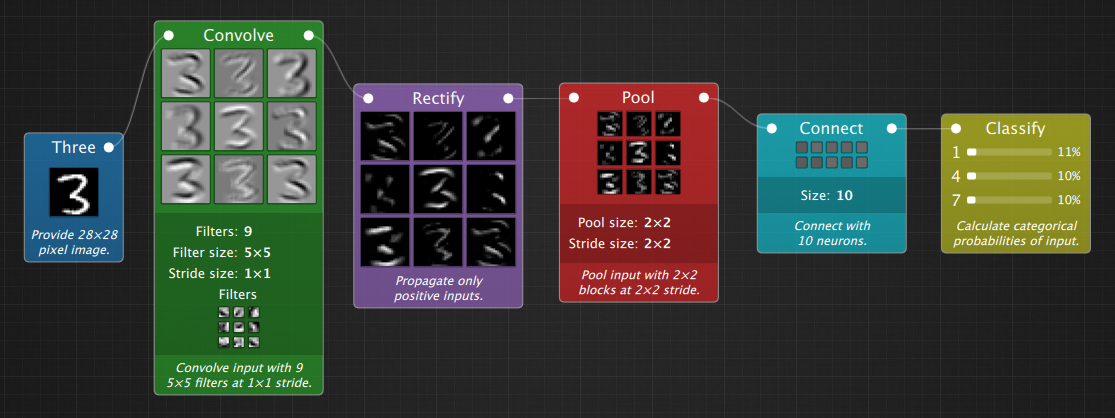
\includegraphics[scale=0.57]{UI/Network}
  \caption{Užitočný nezmysel}
\end{sidewaysfigure}

% ZÁVER

\chapter*{Záver}
\addcontentsline{toc}{chapter}{Záver}

Cieľom výskumu v oblasti umelej inteligencie, je vytvoriť umelú myseľ. Táto myseľ sa musí správať ako dokonalá čierna skrinka -- žiadne nastaviteľné parametre, žiadne ladenie a žiadne vnútorné zásahy. Skutočne samostatný \emph{mysliaci stroj}.

Aby sme takýto stroj mohli vytvoriť, potrebujeme nástroje, ktoré nám pomôžu vytvárať a pochopiť systémy založené na umelých neurónových sieťach. Takéto prostredie nám musí ponúkať tri druhy reprezentácií -- enaktívne, ikonické a symbolické. Tieto reprezentácie musia byť vzájomne prepojené, aby poskytovali čo najbohatší obraz o vytváranom systéme.

Vizuálne programovanie doplnené o zobrazovanie spracovávaných dát je prostredie, ktoré nám umožní široké spektrum experiementovania s neurónovými sieťami. Vďaka takémuto prostrediu budeme môcť vidieť, čo neurónová sieť robí a ako sa správa. Nebudeme si ju musieť simulovať v hlave na inej neurónovej sieti.
 
Na to aby sme vytvorili skutočnú čiernu skrinku, najskôr potrebujeme do nej jasne vidieť. Až potom ju môžeme natrieť na čierno.

\vfill

\begin{quote}
  \Large
We can only see a short distance ahead, but we can see plenty there that needs to be done.\\
\mbox{}~\hfill \large Alan Turing
\end{quote}

\vfill

% záverečná časť
\backmatter{}

% literatúra
\printbibliography[heading=bibnumbered]

% príloha
\appendix
\chapter{Príloha}

Túto publikáciu, zdrojové kódy prototypu a dodatočné materiály je možné nájsť na~ webovej adrese \url{http://github.com/mlajtos/MasterThesis}.

\vfill

\begin{center}
  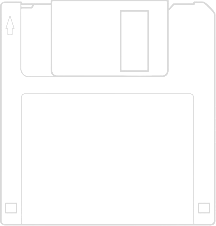
\includegraphics[width=10cm]{Disketa}  
\end{center}

\vfill

Tento digitálny nosič je prázdny. Slúži iba ako pripomienka, že všetky médiá majú obmedzenú životnosť.

\vfill

\end{document}
			